%!TEX root = ./../../thesis-format/main.tex

Here, we investigate classes of transformations.
Sections~\ref{prelim:sec:perm}, \ref{prelim:sec:cycles}, \ref{subsec:tail}, \ref{prelim:sec:oneattractor}, and~\ref{prelim:sec:idempotent}
introduce and investigate permutations, cycles, one-point singulars, and idempotent transformations, respectively.
In \cref{prelim:sec:idempotentoneattractor},
we investigate idempotent one-singulars.
We will present different characterizations.
Later, the transformations that arise  in the study of automata theory
result from compositions of transformations induced by letters.
For this reason, we also investigate
resulting transformations when composing different types of transformations.

\section{Permutations and Quasipermutations} 
\label{prelim:sec:perm} 

%!TEX root = ./../../springer-mono-format/book.tex
%!TEX root = ./../../thesis-trier.tex

\IN{permutation}
\IN{inverse transformation}
A \emph{permutation} is a bijective transformation.
Recall that, in this case, as discussed in \cref{prelim:subsec:func:basic}, 
there exists an \emph{inverse transformation} $t^{-1} \colon X \to X$
such that $\concat{t}{t^{-1}} = \concat{t^{-1}}{t} = \operatorname{id}_X$.


\IN{permuted subset} 
\IN{quasipermutation}
For an arbitrary transformation $t \colon X \to X$
and $S \subseteq X$ we say that $t$ \emph{permutes a subset $S \subseteq X$} 
if $t_{|S}$ is a permutation on $S$. 
We call~$t \colon X \to X$ a \emph{quasipermutation}~\cite{GorKou95} if it permutes its image $t(X)$.

First, in~\cref{prelim:prop:permutation} we collect several well-known characterizations of permutations
on finite sets. Then, the remaining statements investigate quasipermutations.

\begin{proposition}
	\label{prelim:prop:permutation} \label{prelim:prop:non-perm-dupl-cycle}
	Let $t \colon [n] \to [n]$. Then the following are equivalent.
	\begin{enumerate}
		\item \label{prelim:prop:item:not_perm} $t$ is a permutation.
		
		\item \label{prelim:prop:item:non_injective} $\dupl{t} = \emptyset$, i.e., $t$ is injective.		
		
		\item \label{prelim:prop:item:invdupl} $t^{-1}(\dupl{t}) \cap t([n])$ is empty.
				
		\item \label{prelim:prop:item:root} $t$ has no root point.
				
		\item \label{prelim:prop:item:defect} $\defect{t} = 0$.
		
		\item \label{prelim:prop:item:cycles} Every state is a cycle state.
		
		\item \label{prelim:prop:item:identity} There exists $i > 0$ such that $t^i = \operatorname{id}_{[n]}$.			
		
		\item \label{prelim:prop:item:not_surjective} $\rank{t} = n$, i.e., $t$ is surjective.		
	\end{enumerate}	
\end{proposition}
\begin{proof} 
	$\ref{prelim:prop:item:not_perm}\Rightarrow~\ref{prelim:prop:item:non_injective}$: This follows as a permutation 
	is injective by definition.
		
	$\ref{prelim:prop:item:non_injective}\Rightarrow~\ref{prelim:prop:item:invdupl}$: 
	This is obvious.
	
	$\ref{prelim:prop:item:invdupl}\Rightarrow~\ref{prelim:prop:item:root}$:
	Let $y \in [n]$ be a root point.
	Then $y \in \dupl{t}$ and $t^p(y) = y$ for some $p > 0$.
	This gives $t^{p-1}(y) \in t^{-1}(\dupl{t}) \cap t([n])$.	
		
	$\ref{prelim:prop:item:root}\Rightarrow~\ref{prelim:prop:item:defect}$:
	Suppose $\defect{t} > 0$.
	Then there exists $x \in \excl{t}$.
	By finiteness, there exists a minimal $i \ge 0$
	such that $t^i(x) = t^{i+p}(x)$ for some $p > 0$, where, since $x \in \excl{t}$, we must have $i > 0$.
	Set $y = t^{i}(x)$. We have $t^p(y) = y$.
	By the minimal choice of~$i$, we have $t^{i-1}(x) \ne t^{i + p - 1}(x)$
	and both map to the same point~$y$. Hence we have $y \in \dupl{t}$.
	Thus~$y$ is a root point.
		
	$\ref{prelim:prop:item:defect}\Rightarrow~\ref{prelim:prop:item:cycles}$:
	By \cref{prelim:prop:item:defdupl2} from~\cref{prelim:prop:gentransdef},
	we have $|\dupl{t}| \le \defect{t} = 0$, i.e.~$t$ is injective.
	By finiteness
	there exist $i \ge 0$ and $p > 0$ with $i$ minimal
	such that $t^i(x) = t^{i+p}(x)$.
	For $i > 0$, by injectivity, we obtain $t^{i-1}(x) = t^{i - 1 + p}(x)$,
	contradicting the minimal choice of $i$. So $i = 0$ and $x = t^p(x)$. Thus~$x$
	is a cycle state.
		
	$\ref{prelim:prop:item:cycles}\Rightarrow~\ref{prelim:prop:item:identity}$: 
	By assumption for each $x \in [n]$ there exists $i_x > 0$
	such that $\applyfunc{x}{t^{i_x}} = x$.
	Then $t^{\lcm\{ i_x \mid x \in [n] \}} = \operatorname{id}_{[n]}$.	
	
	$\ref{prelim:prop:item:identity}\Rightarrow~\ref{prelim:prop:item:not_surjective}$: 
	By assumption we have $x = t(t^{i-1}(x)) \in t([n])$ for each $x \in [n]$.
	So $t([n]) = [n]$, which gives $\rank{t} = n$.	
	
	$\ref{prelim:prop:item:not_surjective}\Rightarrow~\ref{prelim:prop:item:not_perm}$:
	By \cref{prelim:prop:item:rank-defect-eqn} from \cref{prelim:prop:rank-defect} 
	we have $n = \rank{t} = n + \defect{t}$. Thus $\defect{t} = 0$.
	By \cref{prelim:prop:item:defdupl2} from~\cref{prelim:prop:gentransdef},
	we have $|\dupl{t}| \le \defect{t} = 0$, i.e.~$t$ is injective.	
\end{proof} 

\begin{corollary}
    Let $t \colon X \to X$ and $S \subseteq X$ be finite.
    Then~$t$ permutes~$S$ if and only if $t(S) = S$.		
\end{corollary}

\begin{proposition} \label{prelim:prop:quasiperm}
	Let $t \colon [n] \to [n]$. Then the following are equivalent.
	\begin{enumerate}
		\item \label{prelim:prop:quasiperm:1} $t$ is a quasipermutation.	
		
		\item \label{prelim:prop:quasiperm:2} For each $x \in X$, $t(x)$ is a cycle point.
		
		\item \label{prelim:prop:quasiperm:3} For each $x \in \excl{t}$, $t(x)$ is a cycle point.	
		
		\item \label{prelim:prop:quasiperm:4} The set of tail points equals $\excl{t}$.
		
		\item \label{prelim:prop:quasiperm:5} $\dupl{t_{|t([n])}} = \emptyset$.
		
		% noch: t^{-1}(dupl) nur excl und cycle states
	\end{enumerate}	
\end{proposition}
\begin{proof}
	$\ref{prelim:prop:quasiperm:1}\Rightarrow \ref{prelim:prop:quasiperm:2}$:
	By assumption, $t_{|t(X)}$ is a permtuation.
	Then the claim follows from \cref{prelim:prop:item:cycles} of \cref{prelim:prop:permutation}
	applied to the permutation $t_{|t(X)}$.
		
	$\ref{prelim:prop:quasiperm:2}\Rightarrow \ref{prelim:prop:quasiperm:3}$:	This is clear.
		
	$\ref{prelim:prop:quasiperm:3}\Rightarrow \ref{prelim:prop:quasiperm:4}$:	
	Clearly, states in $\excl{t}$ are tail points.
	For a tail point $x$ we have $x = t^i(z)$
	for an excluded point~$z$ and some $i \ge 0$.
	By assumption, $i = 0$ and so $x = z$.
	Thus $\excl{t}$ equals precisely the tail points.	
	
	$\ref{prelim:prop:quasiperm:4}\Rightarrow \ref{prelim:prop:quasiperm:5}$:
	Assume $t_{|t(X)}$ is not injective.
	Then $t(t(x)) = t(t(z))$ for $x,z \in [n]$
	with $t(x) \ne t(z)$.
	Since a cycle point has precisely one predecessor on its cycle,
	one of both points $t(x)$ or $t(z)$ must be a tail point,
	and this point is $t(X)$.
	
	$\ref{prelim:prop:quasiperm:5}\Rightarrow \ref{prelim:prop:quasiperm:1}$:
	We have $t(t([n])) \subseteq t([n])$.
	By assumption, $t$ acts injectively on $t(X)$.
	This yields $|t(t([n]))| = |t([n])|$ and thus we 
	obtain $t(t([n])) = t([n])$.
\end{proof}

\begin{lemma} \label{prelim:trans:lem:stable-fibers}
	Let $t \colon [n] \to [n]$ be a quasipermutation. Then
	\[
	|t^{-1}(y)| = |t^{-1}(y) \cap \excl{t}| + 1
	\quad \text{for } y \in t([n]),
	\]
	and $t^{-1}(y) = \emptyset$ otherwise. In particular
	$\dupl{t} = t(\excl{t})$.
\end{lemma}
\begin{proof}
	As $t(t([n])) = t([n])$ and $t([n])$ is finite, $t_{|t([n])}$ is a permutation
	of $t([n])$. Hence every $y \in t([n])$ has exactly one preimage in $t([n])$,
	and the remaining preimages lie in $\excl{t} = [n] \setminus t([n])$, which
	gives the displayed equality; points outside $t([n])$ have no preimage.
	Consequently $|t^{-1}(y)| \ge 2$ if and only if $t^{-1}(y)$ meets $\excl{t}$,
	that is, if and only if $y \in t(\excl{t})$.
\end{proof}

\begin{proposition}
	Let $t \colon [n] \to [n]$ be of defect at most two.
	If $\dupl{t} = t(\excl{t})$, then~$t$ is a quasipermutation. 
\end{proposition}
\begin{proof}
	If there exists $x \in \dupl{t}$
	not contained in a cycle, then $x = t^i(y) = t^j(z)$
	for two distinct excluded points $y, z \in \excl{t}$ and $i,j \ge 1$.
	By \cref{prelim:prop:item:root} of \cref{prelim:prop:non-perm-dupl-cycle} 
	there exists another point in $\dupl{t}$ contained in a cycle,
	which must be the image of yet another excluded point by assumption.
	Then $t$ would have defect at least three.
	Thus every duplicate point is contained in a cycle.
	Then, with $\dupl{t} = t(\excl{t})$,
	the image of every excluded point is a cycle point.
	Thus, with \cref{prelim:prop:quasiperm}, $t$ is a quasipermutation.	
\end{proof}

\section{Cycles and Cycles Induced by a Transformation} 
\label{prelim:sec:cycles}

%!TEX root = ./../../thesis-trier.tex

\index{$m$-cycle|see{cycle}} 
\IN{cycle} 
\index{cyclic permutation|see {cycle}} 
\IN{cyclically permuting a set}
\IN{transposition}
\IN{cycle notation} \label{def:cycle-notation}
\IN{disjoint cycles}
\IN{cycle induced by transformation}
\IN{cycle contained in transformation!see {cycle induced by transformation}}
\IN{permuted subset}
\IN{point contained in cycle}
Let $X$ be some set and $a_0, a_1, \ldots, a_{m-1} \in X$ be $m \ge 1$ distinct elements.
Then the permutation $(a_0 ~ a_1 ~ \cdots ~ a_{m-1})_X \colon X \to X$ 
given by 
\[
(a_0 ~ a_1 ~ \cdots ~ a_{m-1})_X(x) = 
\begin{cases} 
	a_{(j+1) \bmod m} & \text{if } x = a_j \text{ for some } j \in \{0,1,\ldots,m-1\}, \\
	x & \text{otherwise,}
\end{cases} 
\]
is called an \emph{$m$-cycle} or \emph{cycle} of length $m$.\footnote{Note that for $X \ne \{a_0,a_1, \ldots, a_m\}$
	the cycle has fixpoints. Some authors exclude this possibility and 
	stipulate $X = \{a_0,a_1, \ldots, a_m\}$.}

Equivalently, $t \colon X \to X$ is an $m$-cycle if and only if
$m \le 1$ and $t = \operatorname{id}_X$ 
or $m = |\move{t}|$ and for $x,x' \in \move{t}$
there exists $i \ge 0$
such that $t^i(x) = x'$.
When the context is clear, we often omit the index~$X$ and simply write $(a_0 ~ a_1 ~ \cdots ~ a_{m-1})$.
We do not use commas in the cycle notation between points, 
to distinguish it from an ordinary $m$-tuple.
When writing a $1 \times n$ matrix as in \cref{prelim:sync_max:matrixscheme} 
we obtain the same notation as for a cycle,
but in each case the context should make it clear whether we refer to a cycle or a $1 \times n$ matrix.
For each $a \in X$, we have $(a) = () = \operatorname{id}_X$.
The following equations hold:
\begingroup
\allowdisplaybreaks 
\begin{align}
	(a_0 ~ a_1  ~\cdots~  a_{m-2} ~ a_{m-1}) & = (a_1 ~ a_2 ~ \cdots ~ a_{m-1} ~ a_0) \\
	(a_0 ~ a_1  ~\cdots~  a_{m-1}) & = (a_1 ~\cdots~ a_{m-1})(a_0 ~ a_{m-1}) = (a_0 ~ a_2 ~ \cdots ~ a_{m-1}) (a_0 ~ a_1) \label{prelim:eqn:cycletrans1} \\
	(a_0 ~ a_1  ~\cdots~  a_{m-1}) & = (a_{m-2} ~ a_{m-1})(a_0 ~ a_1  ~\cdots~  a_{m-3} ~ a_{m-1}) \label{prelim:eqn:cycletrans2} \\		
	(a_0 ~ a_1  ~\cdots~  a_{m-1}) & = (a_0 ~ a_1)( a_1 ~\cdots~ a_{m-1}) \\		
	(a_0 ~ a_1  ~\cdots~ a_{m-2} ~ a_{m-1}) & = \concat{\concat{(a_0 ~\cdots~ a_{m-3})}{(a_{m-2} ~ a_{m-1})}}{(a_{m-2} ~ a_0)} 
\end{align}
\endgroup%
% einige oben nur spezialfälle davon
And for $0 \le i < j < m$ we have:
\begin{align*}
	(a_0 ~ a_1 ~\cdots~ a_{m-1})(a_i ~ a_j)
	& = (a_0 ~ a_1 ~\cdots~ a_{i} ~ a_{j+1} ~ a_{j+1} \cdots a_{m-1})(a_{i+1} ~\cdots ~ a_j) \\
	(a_i ~ a_j)(a_0 ~ a_1 ~\cdots~ a_{m-1})
	& = (a_0 ~ a_1 ~\cdots~ a_{i-1} ~ a_j ~ a_{j+1} ~\cdots~ a_m)(a_i ~ \cdots ~ a_{j-1})
\end{align*}

A \emph{transposition} is a $2$-cycle. Two cycles~$t,h \colon X \to X$ are \emph{disjoint} if $\move{t} \cap \move{h} = \emptyset$,
in this case we have $th = ht$.  
Let $t \colon X \to X$ be some transformation.
For finite $S \subseteq X$, we say that $t$
\emph{cyclically permutes $S$} if $t$ permutes $S$
and $t_{|S}$ is an $|S|$-cycle. 
Then $t^{|S|}(x) = x$ for all $x \in S$. A permutation on a set of size at least two cyclically permutes its domain
if and only if it is a cycle with no fixpoints.
If $t_{|S} = (a_0 ~ a_1 ~ \ldots ~ a_{m-1})$
we also say that $t$ 
\emph{induces the cycle}, or \emph{contains the cycle}, $(a_0 ~ a_1 ~ \cdots ~ a_{m-1})$.
Equivalently, $t(a_j) = a_{(j+1) \bmod m}$ for all $j \in \{0,1,\ldots,m-1\}$, i.e.,
$(x ~ t^2(x) ~ \cdots ~ t^{m-1}(x)) = (a_0 ~ a_1 ~ \ldots ~ a_{m-1})$.
%Then, for each $x \in \{a_0, a_1, \ldots, a_{m-1}\}$,
%we have $t^m(x) = x$. Conversely, 
For $x \in X$ and $m \ge 1$, the points 
$x, t(x), \ldots, t^{m-1}(x)$ form a cycle induced by $t$ if and only if~$m$ is minimal
such that $t^m(x) = x$.
Two distinct cycles induced by $t$ are disjoint.

\begin{proposition} \label{prelim:fact:product_disjoint_cycles} 
	A permutation on a finite set equals the composition (in any order) of its induced cycles.	
\end{proposition}
\begin{proof}
	Let~$t \colon [n]\to [n]$ be a permutation
	with induced cycles $t_1, \ldots, t_m$.
	For $x \in [n]$, we have $t_i = (x ~ t(x) \cdots t^{k-1}(x))$
	for some minimal $k \ge 1$ with $t^k(x) = x$ and 
	unique $i \in \{1,\ldots,m\}$.
	Furthermore, for $j \ne i$, we also have $t_j(x) = x$.
	Thus, the result of any composition of
	$t_1, \ldots, t_m$ maps $x$ to $t_i(x) = t(x)$,
	and so this composition equals~$t$.
\end{proof}

\begin{corollary} \label{prelim:fact:transpositions_generate_Sn}
	A permutation on a finite set can be written as
	a composition of transpositions.
\end{corollary}
\begin{proof}
	This follows from \cref{prelim:eqn:cycletrans1,prelim:fact:product_disjoint_cycles}.
\end{proof}

\section{Tail Transformations, Simple Idempotents, and Cycles}
\label{subsec:tail}

%!TEX root = ./../../springer-mono-format/book.tex
%!TEX root = ./../../thesis-trier.tex

Here, we introduce tail transformations and simple idempotents.
We then classify the transformations obtained by composing a simple idempotent with a cycle.
\cref{constrsync:prop:concat_cycle_SI} bounds
the length of cycles induced in the composition of a simple idempotent with a cycle.

\IN{simple idempotent}
\IN{singular transformation|see{simple idempotent}}
\IN{tail transformation}
Let $a_1, \ldots, a_m \in X$ be distinct numbers with $m \ge 2$. The \emph{tail transformation (of $a_1,\ldots a_m$)}
is the transformation $[a_1 \mapsto a_2 \mapsto \cdots \mapsto a_m]_X \colon X \to X$
given by   \label{def:SI-mapping}
\[
\applyfunc{x}{[a_1 \mapsto a_2 \mapsto \cdots \mapsto a_m]_X} = 
\begin{cases}
	a_{i+1} & \text{if } x = a_i \text{ for } i \in \{1,\ldots,m-1\}, \\ 
	x       & \text{otherwise.}
\end{cases}
\]
When the context is clear, we often omit $X$ and simply write $[a_1 \mapsto a_2 \mapsto \cdots \mapsto a_m]$.

\begin{proposition} \label{prelim:prop:tail-comp} \label{prelim:trans:eqn:SI-one-singular}
	Let $a_1, \ldots, a_m \in X$ be pairwise distinct and $1 < i < m$. Then
	\begin{align*}
		[a_1 \mapsto a_2 \mapsto \cdots \mapsto a_m] 
		& = \concat{[a_i \mapsto a_{i+1} \mapsto \cdots \mapsto a_m]}{[a_1 \mapsto a_2 \mapsto \cdots \mapsto a_i]} \\
		t \SI{a_i}{a_{i-1}} = \SI{a_i}{a_{i+1}}t & = \concat{[a_1 \mapsto a_2 \mapsto \cdots \mapsto a_i]}{[a_i \mapsto a_{i+1} \mapsto \cdots \mapsto a_m]} 
	\end{align*}
	where $t = [a_1 \mapsto a_2 \mapsto \cdots a_{i-1} \mapsto a_{i+1} \mapsto \cdots \mapsto a_m]$.
\end{proposition}

A \emph{simple idempotent} is a tail transformation involving two distinct numbers, i.e., where $m = 2$.\footnote{Also called a \emph{singular} transformation in~\cite{DBLP:journals/ijfcs/Brzozowski13}.}
So, a simple idempotent is written as $\SI{a}{b}$ for distinct $a,b \in X$.
In~\cite{CameronRGM2017} a similar notation was used.
A transformation $t \colon X \to X$ is a simple idempotent if and only if $\move{t}$ is a singleton set.

\begin{proposition} \label{prelim:trans:prop:SI-relations}
	For pairwise distinct $a,b,c,d \in X$, the following equations hold:
	\begingroup
	\allowdisplaybreaks 
	\begin{align}
		\concat{\SI{a}{b}}{\SI{a}{b}} & = \SI{a}{b} = \concat{\SI{b}{a}}{\SI{a}{b}} \label{prelim:trans:eqn:SI-itself} \\
		\concat{\SI{a}{b}}{\SI{c}{d}} & = \concat{\SI{c}{d}}{\SI{a}{b}} \label{prelim:tran:eqn:SI-all-distinct} \\
		\concat{\SI{a}{b}}{\SI{a}{c}} & = \SI{a}{b} \label{prelim:tran:eqn:SI-common-start} \\
		\concat{\SI{a}{b}}{\SI{c}{b}} & = \concat{\SI{c}{b}}{\SI{a}{b}} = \concat{\SI{c}{a}}{\SI{a}{b}} \label{prelim:trans:eqn:SI-one-singular0} \\
		\concat{\SI{b}{c}}{\concat{\SI{a}{b}}{\SI{c}{a}}} & = \concat{\concat{\SI{c}{b}}{\SI{a}{c}}}{\concat{\SI{b}{a}}{\SI{c}{b}}} \\
		\concat{\SI{b}{c}}{\concat{\SI{a}{b}}{\concat{\SI{c}{a}}{\SI{d}{c}}}} & = 
		\concat{\SI{c}{b}}{\concat{\SI{d}{c}}{\concat{\SI{b}{d}}{\concat{\SI{a}{b}}{\SI{d}{a}}}}}
	\end{align}
	\endgroup%
\end{proposition}

\Cref{prelim:trans:eqn:SI-one-singular0} also follows from \cref{prelim:prop:tail-comp} for $m = 3$,
but is kept for reference.
The equations from \cref{prelim:trans:prop:SI-relations} yield a presentation
in terms of generators and relations for the set of all non-permutations on a finite set~\cite{East2013}.

\begin{corollary}
	Let $a,b,c,d \in X$ with $a \ne b$ and $c \ne d$ and $\SI{a}{b} \ne \SI{c}{d}$.
	Then
	we have 
	$\concat{\SI{a}{b}}{\SI{c}{d}} 
	= \concat{\SI{c}{d}}{\SI{a}{b}}$
	if and only if $a \ne c$ and $b \ne c$ and $d \ne a$, i.e., 
	both simple idempotents commute if and only if $a,b,c,d$ are all distinct
	or $b = d$ and $a,b,c$ are all distinct.
\end{corollary}
\begin{proof}
	For $a = c$, since $\SI{a}{b} \ne \SI{c}{d}$
	we have $d \ne b$
	and both simple idempotents
	do not commute by \cref{prelim:tran:eqn:SI-common-start}.
	Next, suppose $b = c$.
	For $a = d$,
	both do not commute by \cref{prelim:trans:eqn:SI-itself}.
	For $a \ne d$,
	we have $\concat{\SI{c}{d}}{\SI{a}{c}} = [a \mapsto c \mapsto d] \ne \concat{\SI{a}{c}}{\SI{c}{d}}$.
	
	Conversely, suppose $a \ne c, b \ne c, d \ne a$, i.e., $a \notin \{c,d\}$ and $b \ne c$.
	If $b \ne d$, i.e., all points are pairwise distinct,
	we have $\SI{a}{b}\SI{c}{d} = \SI{c}{d}\SI{a}{b}$ by \cref{prelim:tran:eqn:SI-all-distinct}.
	For $b = d$, we have $\SI{a}{b}\SI{c}{b} = \SI{c}{b}\SI{a}{b}$
	by \cref{prelim:trans:eqn:SI-one-singular0}.
\end{proof}

Let $t = \SI{a}{b}$ for $a \ne b$. Then $\dupl{t} = \{b\}$, $\excl{t} = \{a\}$, and 
for finite $S \subseteq X$ we have
\begin{align}
	|t(S)| < |S| & \Leftrightarrow \{a,b\} \subseteq S \Leftrightarrow S = t(S) \cup \{a\}, \label{prelim:eqn:SIsmaller} \\
	|t(S)| = |S| & \Leftrightarrow t(S) = S \lor ( b \notin S \land a \in S \land t(S) = ( S \cup \{b\} ) \setminus \{a\} ). \label{prelim:eqn:SIequalsize}
\end{align}

The following equations encompass, up to a renaming of the points,
all combinations to compose a simple idempotent with a cycle.
\Cref{prelim:eqn:SIcycle1,prelim:eqn:SIcycle2}
are illustrated in \cref{prelim:fig:composition-cycle-SI}.

\begin{proposition} \label{prelim:trans:prop:cycle-SI-composition}
	Let $m \ge 2$, $\{0,1,\ldots,m\} \subseteq X$,
	and $0 < d \le m$. Then we have
	\begin{align}
		[0 \mapsto d ](0 ~ 1 ~\cdots ~ m) 
		& = [0 \mapsto \cdots \mapsto d - 1 \mapsto d](d ~ d+1 ~ \cdots ~ m)  \label{prelim:eqn:SIcycle1} \\
		& = (d ~ d+1 ~ \cdots ~ m)[0 \mapsto \cdots \mapsto d - 1 \mapsto m] \\
		& = \concat{[m\mapsto d]}{(0 ~ 1 ~ \cdots ~ m)} \\
		& = \concat{[0 \mapsto 1 \mapsto \cdots \mapsto m]}{[m\mapsto d]} \\
		& = \concat{[m\mapsto d-1]}{[0 \mapsto 1 \mapsto \cdots \mapsto m]}
	\end{align}
	and for distinct $a,b \in X \setminus \{0,1,\ldots,m\}$ we have
	\begin{align}
		(0 ~ 1 ~\cdots ~ m)[ 0 \mapsto d ] & = [1 \mapsto 2 \mapsto \cdots \mapsto d+1](0 ~ d + 1 ~ \cdots ~ m) \label{prelim:eqn:SIcycle2} \\
		(0 ~ 1 ~ \cdots ~ m)[0 \mapsto a] & = [1 \mapsto \cdots \mapsto m \mapsto 0 \mapsto a] \label{prelim:eqn:SIcycle4} \\
		[0 \mapsto a](0 ~ 1 ~ \cdots ~ m) & = [0 \mapsto 1 \mapsto \cdots \mapsto m \mapsto a] \label{prelim:eqn:SIcycle5} \\
		(0 ~ 1 ~ \cdots ~ m)\SI{a}{b} & = \SI{a}{b}(0 ~ 1 ~ \cdots ~ m) \label{prelim:eqn:SIcycle6}
	\end{align} 
\end{proposition}

\begin{corollary} For $m \ge 2$ we have the following:
	\[
		[0 \mapsto 1](0 ~ 1 ~ \cdots ~ m) 
		= [0 \mapsto 1 ](1 ~ 2 ~ \cdots ~ m) 
		= (1 ~ 2 ~ \cdots ~ m)[ 0 \mapsto m] 
		= \concat{[m \mapsto 0]}{(0 ~ 1 ~ \cdots ~ m)}
	\]
\end{corollary}

\begin{figure}[ht]
	\centering
	\begin{subfigure}{0.45\textwidth}
		\centering
		\scalebox{1.0}{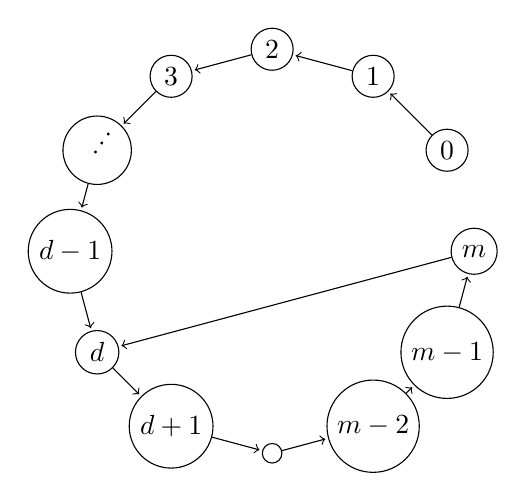
\begin{tikzpicture}[shorten >=1pt,->,node distance=4cm]
				%\tikzstyle{vertex}=[circle,color=red!60,fill=black!10,minimum size=25pt,inner sep=1pt,very thick]
				%\tikzstyle{vertex}=[circle,draw,minimum size=5pt,inner sep=1pt]
				
				% state,blur shadow, fill={rgb:black,0.4;white,10}, inner sep=0pt, minimum size=35pt
				
				\foreach \name/\angle/\text in {P0/0/m,P1/30/0,P2/60/1,P3/90/2,P4/120/3,
					P6/180/d-1,P7/210/d,P8/240/d+1,P9/300/m-2,P10/330/m-1}
				\node (\name) at (\angle:7.3em) {$\text$};  %{\small $\text$};
				
				
				\node (D) at (150:7.3em) {\rotatebox{145}{$\vdots$}}; 
				\node (D2) at (270:7.3em) {$\hdots$};				
				
				\path[->] (P0) edge (P7);
				\path[->] (P7) edge (P8);
				\path[->] (P8) edge (D2);
				\path[->] (D2) edge (P9);
				\path[->] (P9) edge (P10);
				\path[->] (P10) edge (P0);
				\path[->] (P1) edge (P2);
				\path[->] (P2) edge (P3);
				\path[->] (P3) edge (P4);
				\path[->] (P4) edge (D);
				\path[->] (D) edge (P6);
				\path[->] (P6) edge (P7);				
		\end{tikzpicture}}
		\caption{$\concat{(0 ~ 1 ~ \cdots ~ m)}{[ 0 \mapsto d ]}$.}
	\end{subfigure}
	\begin{subfigure}{0.45\textwidth}
		\centering
		\scalebox{1.0}{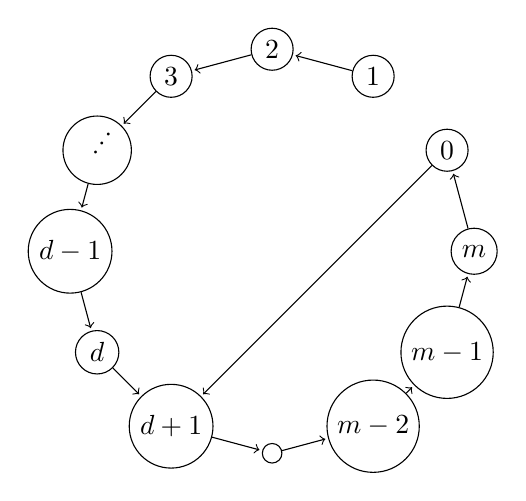
\begin{tikzpicture}[shorten >=1pt,->,node distance=4cm]				
				\foreach \name/\angle/\text in {P0/0/m,P1/30/0,P2/60/1,P3/90/2,P4/120/3,
					P6/180/d-1,P7/210/d,P8/240/d+1,P9/300/m-2,P10/330/m-1}
				\node (\name) at (\angle:7.3em) {$\text$};  %{\small $\text$};
				
				\node (D) at (150:7.3em) {\rotatebox{145}{$\vdots$}}; 
				\node (D2) at (270:7.3em) {$\hdots$};
				
				\path[->] (P0) edge (P1);
				\path[->] (P7) edge (P8);
				\path[->] (P8) edge (D2);
				\path[->] (D2) edge (P9);
				\path[->] (P9) edge (P10);
				\path[->] (P10) edge (P0);
				\path[->] (P1) edge (P8);
				\path[->] (P2) edge (P3);
				\path[->] (P3) edge (P4);
				\path[->] (P4) edge (D);
				\path[->] (D) edge (P6);
				\path[->] (P6) edge (P7);
		\end{tikzpicture}}
		\caption{$\concat{[ 0 \mapsto d ]}{(0 ~ 1 ~ \cdots ~ m)}$.}
	\end{subfigure}
	\caption[Composition of cycle and simple idempotent]{Functional graphs resulting from the two possible compositions of $(0 ~ 1 ~ \cdots ~ m)$
		with $\SI{0}{d}$ where $0 < d \le m$, see \cref{prelim:eqn:SIcycle1,prelim:eqn:SIcycle2}.}
	\label{prelim:fig:composition-cycle-SI}
\end{figure}

\begin{corollary} \label{constrsync:prop:concat_cycle_SI}	
	Let $t \colon X \to X$ be an $m$-cycle
	and $h \colon X \to X$ be a simple idempotent.
	Then there exist $0 \le i,j \le m$
	and $0 < p,q < m$
	such that $( \concat{t}{h} )^i = ( \concat{t}{h} )^{i + p}$
	and $( \concat{h}{t} )^j = ( \concat{h}{t} )^{j+q}$.
\end{corollary}
\begin{proof}
	We can assume $m \ge 2$.
	This follows from the equations given in \cref{prelim:trans:prop:cycle-SI-composition}, since
	the results of both compositions move at most $m + 2$ points,
	contain at most one cycle moving more than one point, and such a cycle moves at most~$m$
	points, or it equals a tail transformation moving at most $m + 1$ 	points.	
\end{proof}

\section{One-Point Singular Transformations}
\label{prelim:sec:oneattractor} 

%!TEX root = ./../../springer-mono-format/book.tex
%!TEX root = ./../../thesis-trier.tex

\IN{one-point singular}
A transformation $t \colon X \to X$ 
is said to be \emph{one-point singular}~\cite{Rystsov2024}
if $\dupl{t}$ is a singleton. 
As a slight abuse of language, using an adjective as a noun, we call
a one-point singular transformation simply a one-point singular.

To give a few examples, simple idempotents
and, by  \crefitem{prelim:prop:gentransdef}{prelim:prop:item:defdupl2},
defect-one transformations on finite sets are one-point singulars.
\Cref{prelim:trans:fig:onepointsing} depicts the functional graph
of an example one-point singular.

\Cref{prop:char-one-attractor0,prop:char-one-attractor}
provide characterizations of transformations
that are injective or one-point singulars,
the latter investigating the case of a finite domain.
\Cref{prelim:trans:cor:char-one-point-singular} gives a characterization
in the special case of quasipermutations.
\Cref{prelim:prop:comp-one-point-singular-cases}
characterizes when the composition of two transformations
gives a one-point singular. The special case when both transformations
are one-point singulars is given in \cref{prelim:cor:comp-one-point-singulars}.

\begin{figure}[ht]
	\centering
	\begin{tikzpicture}
		\tikzset{every node/.style={draw,circle,inner sep=2.5pt}}
		
		\def\radius{2cm}
		\def\shiftX{5cm}
		\def\nA{10}
		\def\nB{8}
		
		\foreach \i in {1,...,\nA} {
			\node (A\i) at ({\radius*cos(360/\nA * \i)}, {\radius*sin(360/\nA * \i)}) {};
		}
		
		\foreach \i in {2,...,\nA} {
			\path[->] (A\the\numexpr\i-1\relax) edge (A\i);
		} 
		\path[->] (A\nA) edge (A1);
		
		\foreach \j in {1,...,\nB} {
			\node (B\j) at ({\shiftX + 0.8*\radius*cos(360/\nB * \j)}, {0.8*\radius*sin(360/\nB * \j)}) {};
		}				
		
		\foreach \i in {2,...,\nB} {
			\path[->] (B\the\numexpr\i-1\relax) edge (B\i);
		} 
		\path[->] (B\nB) edge (B1);
		
		\node[above = of A4] (T11) {};
		\node[left = of T11] (T12) {};
		\node[left = of T12] (T13) {};
		
		\node[left = of A4] (T21) {};
		
		\node[below left = of A4] (T31) {};
		\node[below = of T31] (T32) {};
		
		\path[->] (T13) edge (T12);
		\path[->] (T12) edge (T11); 
		\path[->] (T11) edge (A4);
		
		\path[->] (T21) edge (A4);
		
		\path[->] (T32) edge (T31);
		\path[->] (T31) edge (A4);
	\end{tikzpicture}
	\caption[Functional graph of a one-point singular]{Functional graph of a one-point singular transformation.}
	\label{prelim:trans:fig:onepointsing}
\end{figure}

\begin{proposition} \label{prop:char-one-attractor0}
 Let $t \colon X \to X$. Then the following are equivalent.	
\begin{enumerate}
\item \label{prop:char-one-attractor0:1} $t$ is injective or a one-point singular.

\item \label{prop:char-one-attractor0:2} for all $x,x',z,z' \in X$,
 if $x \ne x'$, $z \ne z'$, $t(x) = t(x')$, and $t(z) = t(z')$, then $t(x) = t(z)$.
\end{enumerate}
\end{proposition}
\begin{proof}
This follows directly from the definitions.
\end{proof}

\begin{proposition}\label{prop:char-one-attractor}
	Let $t \colon [n] \to [n]$. Then the following are equivalent.
	\begin{enumerate}
		\item \label{prelim:prop:charone:item:one} $t$ is a permutation or a one-point singular.
		
		\item \label{prelim:prop:charone:item:invduple0} $|t^{-1}(\dupl{t})| \le \defect{t} + 1$.
		
		\item \label{prelim:prop:charone:item:invduple} $t$ is a permutation or $|t^{-1}(\dupl{t})| = \defect{t} + 1$. 
		
		\item \label{prelim:prop:charone:item:def1y} There exists $y \in [n]$ such that $|\applyfunc{y}{t^{-1}}| = \defect{t} + 1$.
		
		\item \label{prelim:prop:charone:item:def1} $t$ has kernel type $(\defect{t}+1,1,\ldots,1)$.
		
		\item \label{prelim:prop:charone:item:k111} $t$ has kernel type $(k,1,\ldots,1)$ for some $k \ge 1$.
	\end{enumerate}
\end{proposition}
\begin{proof}
	$\ref{prelim:prop:charone:item:one} \Rightarrow~\ref{prelim:prop:charone:item:invduple0}$:
	By \crefitem{prelim:prop:gentransdef}{prelim:prop:item:defdupl0} we have
	$|t^{-1}(\dupl{t})| = \defect{t} + |\dupl{t}|$.
	Since, by assumption, $|\dupl{t}|\le 1$, we obtain the claim.	
	
	$\ref{prelim:prop:charone:item:invduple0} \Rightarrow~\ref{prelim:prop:charone:item:invduple}$: 
	We have $|t^{-1}(\dupl{t})| = \defect{t} + 1$
	or $|t^{-1}(\dupl{t})| = \defect{t}$.
	In the latter case, from \crefitem{prelim:prop:gentransdef}{prelim:prop:item:defdupl0},
	we get $|\dupl{t}| = 0$. So~$t$ is a permutation.
	 
	$\ref{prelim:prop:charone:item:invduple}\Rightarrow~\ref{prelim:prop:charone:item:def1y}$: Clearly, the implication is true for a permutation. 
	Otherwise, by~\crefitem{prelim:prop:gentransdef}{prelim:prop:item:defdupl0}
	we have $\defect{t} + |\dupl{t}| = |t^{-1}(\dupl{t})| = \defect{t} + 1$.
	So, $|\dupl{t}| = 1$ and 
	$|t^{-1}(y)| = \defect{t} + 1$
	for the unique $y \in \dupl{t}$.
	
	$\ref{prelim:prop:charone:item:def1y} \Rightarrow~\ref{prelim:prop:charone:item:def1}$: Let $y' \in [n] \setminus \{y\}$.
	Then we have
	\begin{align*}
	\defect{t} & \ge |t^{-1}(\{y,y'\})| - 2 \tag{\crefitem{prelim:prop:gentransdef}{prelim:prop:item:defA}} \\
	& = |t^{-1}(y)| + |t^{-1}(y')| - 2 \tag{$|t^{-1}(\{y,y'\})| = |t^{-1}(y)| + |t^{-1}(y')|$} \\
	& = \defect{t} + |t^{-1}(y')| - 1. \tag{$|t^{-1}(y)| = \defect{t} + 1$}
	\end{align*}
	Hence $|t^{-1}(y')| \le 1$.	
	
	$\ref{prelim:prop:charone:item:def1} \Rightarrow~\ref{prelim:prop:charone:item:k111}$ ~ \& ~
	$\ref{prelim:prop:charone:item:k111} \Rightarrow~\ref{prelim:prop:charone:item:one}$: These implications are obvious.
\end{proof}

\begin{proposition} \label{prelim:trans:cor:char-one-point-singular}
	Let $t \colon [n] \to [n]$ be a quasipermutation.
	Then $t$ is a permutation or a one-point singular
	if and only if there exists $y \in [n]$ with $\excl{t} \subseteq t^{-1}(y)$.	
\end{proposition}
\begin{proof}
	By \cref{prelim:trans:lem:stable-fibers} we have $\dupl{t} = t(\excl{t})$.
	By assumption, we have $|\dupl{t}| \le 1$.
	Now $|t(\excl{t})| \le 1$ holds if and only if
	$t(\excl{t}) \subseteq \{y\}$ for some $y \in [n]$, which is
	$\excl{t} \subseteq t^{-1}(y)$.
\end{proof}

\begin{remark} 
	\Cref{prelim:trans:cor:char-one-point-singular}
	might fail if~$t$ is not a quasipermutation.
	For example, let $t \colon \{1,2,3,4\} \to \{1,2,3,4\}$
	with $t(1) = t(3) = 2$ and $t(2) = t(4) = 4$.
	Then $\excl{t} = \{1,3\} \subseteq t^{-1}(2)$,
	but~$t$ has kernel type $(2,2)$.
\end{remark}

%\begin{lemma} \label{prelim:trans:lem:dupl-restr-onepoint}
%	Let $t \colon X \to X$ be one-point singular, let $h \colon X \to X$,
%	and put $Z = t(X) \setminus \dupl{t}$. Then
%	\[
%	\dupl{h_{|t(X)}} = \dupl{h_{|Z}} \cup \bigl( h(\dupl{t}) \cap h(Z) \bigr).
%	\]
%\end{lemma}
%\begin{proof}
%	Apply \cref{prelim:func:eqn:duplicate-partition} to the partition
%	$t(X) = \dupl{t} \cup Z$:
%	\[
%	\dupl{h_{|t(X)}} = \dupl{h_{|\dupl{t}}} \cup \dupl{h_{|Z}}
%	\cup \bigl( h(\dupl{t}) \cap h(Z) \bigr).
%	\]
%	Since~$t$ is one-point singular, $\dupl{t}$ is a singleton set
%	and hence $\dupl{h_{|\dupl{t}}} = \emptyset$.
%\end{proof}
%
%\begin{corollary} \label{prelim:trans:cor:dupl-restr-onepoint}
%	In the situation of \cref{prelim:trans:lem:dupl-restr-onepoint}:
%	\begin{enumerate}
%		\item If $h(\dupl{t}) \cap h(Z) = \emptyset$, then $\dupl{h_{|t(X)}} = \dupl{h_{|Z}}$.
%		\item If $h_{|Z}$ is injective, then $\dupl{h_{|t(X)}} \subseteq h(\dupl{t})$.
%		In particular, as $h(\dupl{t})$ is a singleton set,
%		$\dupl{h_{|t(X)}}$ is either empty or equal to $h(\dupl{t})$.
%	\end{enumerate}
%\end{corollary}




%In the remainder of this section let $t,h \colon X \to X$ and put
%$Z = t(X) \setminus \dupl{t}$.
%Note that a restriction $h_{|Y}$ with $Y \subseteq t(X)$ need not be a
%transformation, as its image need not be contained in~$Y$.
%Moreover, as $\dupl{t} \subseteq t(X)$, injectivity of $h_{|t(X)}$ implies
%$|h(\dupl{t})| = |\dupl{t}|$; in particular, $h(\dupl{t})$ is then a singleton set
%if and only if~$t$ is a one-point singular.
%
%\begin{proposition}  \label{prelim:prop:comp-one-attractor}
%	Let $t,h \colon X \to X$.
%	Then $\concat{t}{h}$ is a one-point singular if and only if exactly one of the
%	following two cases occurs.
%	\begin{enumerate}
%		\item $t$ is injective and $\dupl{h_{|Z}}$ is a singleton set.
%		
%		\item $\dupl{h_{|Z}} \subseteq h(\dupl{t})$ and $h(\dupl{t})$ is a singleton set.
%	\end{enumerate}
%	%	Moreover, $h_{|Z}$ in each case may be replaced independently
%	%	by any subset~$Y$ with $Z \subseteq Y \subseteq t(X)$
%	%	since each case, separately, holds for one such~$Y$ if and only if it holds 
%	%	for every such~$Y$.
%\end{proposition}
%\begin{proof}
%	By \cref{prelim:eqn:dupl} we have $\dupl{\concat{t}{h}} = h(\dupl{t}) \cup \dupl{h_{|Z}}$.
%	Thus, $\dupl{\concat{t}{h}}$ is a singleton set
%	if and only if $\dupl{t} = \emptyset$ and $\dupl{h_{|Z}}$
%	is a singleton set, or if $h(\dupl{t})$ is a singleton set and contains
%	$\dupl{h_{|Z}}$.
%	The two cases are mutually exclusive, since in the second case
%	$h(\dupl{t}) \ne \emptyset$ and hence $\dupl{t} \ne \emptyset$.
%\end{proof}
%
%\begin{remark} \label{prelim:rem:comp-one-attractor}
%	Let $Z \subseteq Y \subseteq t(X)$.
%	Then we have
%	\begin{align*}
%		\text{$t$ is injective} & \Leftrightarrow Z = Y = t(X), \\
%		\dupl{h_{|Z}} \subseteq h(\dupl{t}) & \Leftrightarrow \dupl{h_{|Y}} \subseteq h(\dupl{t}).
%	\end{align*}
%	For the first equivalence, note that~$t$ is injective if and only if
%	$\dupl{t} = \emptyset$, which by $\dupl{t} \subseteq t(X)$ is equivalent to
%	$Z = t(X)$; and then $Y = t(X)$ is the only admissible choice.
%	The second equivalence follows since, by
%	\cref{prelim:func:eqn:duplicate-partition}, we have
%	$
%	\dupl{h_{|Y}} \setminus \dupl{h_{|Z}} \subseteq h(\dupl{t}).
%	$
%	Thus, we can, separately,
%	replace $Z$ by such a set $Y$ in each of the conditions from
%	\cref{prelim:prop:comp-one-attractor},
%	since it holds for some such~$Y$ if and only if it holds for every such~$Y$.
%\end{remark}
%
%\begin{corollary} \label{prelim:cor:comp-one-attractor}
%	Let $t, h \colon X \to X$. Set $B = h(Z) \cap h(\dupl{t})$.
%	Then $\concat{t}{h}$ is a one-point singular if and only if exactly one of the
%	following cases occurs.
%	\begin{enumerate}
%		\item $t$ is injective and $\dupl{h_{|Z}}$ is a singleton set.
%		
%		\item $h_{|t(X)}$ is injective and~$t$ is a one-point singular.
%		
%		\item $B \ne \emptyset$ or $\dupl{h_{|\dupl{t}}} \ne \emptyset$,
%		$h_{|Z}$ is injective, and $h(\dupl{t})$ is a singleton
%		set.\footnote{By \cref{prelim:func:eqn:duplicate-partition}, for injective
%			$h_{|Z}$ we have $B \ne \emptyset$ or $\dupl{h_{|\dupl{t}}} \ne \emptyset$
%			if and only if $h_{|t(X)}$ is not injective.}
%		
%		\item $\dupl{h_{|Z}} = h(\dupl{t})$ and this set is a singleton set.
%	\end{enumerate}
%\end{corollary}
%\begin{proof}
%	By \cref{prelim:prop:comp-one-attractor} it suffices to split its second case,
%	the first one being the first case above.
%	So let $h(\dupl{t})$ be a singleton set.
%	Then $\dupl{h_{|Z}}$, being contained in it, is empty or equal to it, and by
%	\cref{prelim:func:eqn:duplicate-partition} the condition
%	$\dupl{h_{|Z}} \subseteq h(\dupl{t})$ splits into the mutually exclusive cases
%	\begin{enumerate}
%		\item $h_{|t(X)}$ is injective,
%		
%		\item $B \ne \emptyset$ or $\dupl{h_{|\dupl{t}}} \ne \emptyset$, and
%		$h_{|Z}$ is injective,
%		
%		\item $\dupl{h_{|Z}} = h(\dupl{t})$.
%	\end{enumerate}
%	Then the claim follows with the observation that injectivity of $h_{|t(X)}$
%	implies that~$t$ is a one-point singular if $h(\dupl{t})$ is a singleton set.
%\end{proof}
%
%
%
%\begin{remark} \label{prelim:trans:rem:Y-dependence}
%	The condition $\dupl{h_{|Y}} \subseteq h(\dupl{t})$
%	from \cref{prelim:rem:comp-one-attractor} can also be split into the following
%	two conditions:
%	\begin{enumerate}
%		\item \label{prelim:trans:comp-cases:II} $h_{|Y}$ is injective and $h(\dupl{t})$ is a singleton set, or
%		\item \label{prelim:trans:comp-cases:III} $\dupl{h_{|Y}} = h(\dupl{t})$ and this set is a singleton set.
%	\end{enumerate}
%	However, the specific case that applies to a pair $(t,h)$ then depends on~$Y$.
%
%	For example, let $X = \{1,\ldots,5\}$ with
%	$t(1) = t(2) = 1$, $t(3) = t(4) = 2$, $t(5) = 5$ and
%	$h(1) = h(2) = h(3) = 3$, $h(4) = 4$, $h(5) = 5$.
%	Then $\dupl{t} = \{1,2\}$, $Z = \{5\}$, $h(\dupl{t}) = \{3\}$,
%	$\dupl{h_{|Z}} = \emptyset$, $\dupl{h_{|t(X)}} = \{3\}$, and $\concat{t}{h}$
%	maps $1,2,3,4$ to~$3$ and fixes~$5$. So $\dupl{\concat{t}{h}} = \{3\}$, and
%	case~\ref{prelim:trans:comp-cases:II} occurs for $Y = Z$ while
%	case~\ref{prelim:trans:comp-cases:III} occurs for $Y = t(X)$.
%\end{remark}
%
%With \cref{prelim:eqn:dupl0,prelim:eqn:dupl} we also obtain families of statements
%parameterized by a set $Y$ with $Z \subseteq Y \subseteq t(X)$ characterizing
%the composition being one-point singular.
%We state them next. Among these, the last one differs in that its second
%alternative combines the weakest injectivity hypothesis with the strongest
%companion condition.
%Injectivity of $h_{|Y'}$ implies injectivity of $h_{|Y}$ for $Y \subseteq Y'$,
%so the hypothesis is least demanding, and cheapest to verify, for $Y = Z$;
%and~$t$ being a one-point singular implies, but is in general not implied by,
%$h(\dupl{t})$ being a singleton set, the converse holding when $h_{|t(X)}$
%is injective.
%In the third of the statements below the two are tied together, as the strong
%companion condition is available only for $Y = t(X)$, whereas the last statement
%has it for every~$Y$.
%This is paid for in its first alternative, which has to be stated in terms of
%$\dupl{h_{|t(X)}}$ rather than $\dupl{h_{|Y}}$, see
%\cref{prelim:trans:rem:Y-vs-tX}.
%
%\begin{proposition} \label{prelim:trans:prop:comp-criterion}
%	Let $t,h \colon X \to X$, let~$Y$ be a set with $Z \subseteq Y \subseteq t(X)$
%	and put $A = h(\dupl{t})$ and $D_Y = \dupl{h_{|Y}}$. Then the following are
%	equivalent.
%	\begin{enumerate}
%		\item \label{prelim:trans:comp-criterion:1}
%		$\concat{t}{h}$ is a one-point singular.
%		
%		\item \label{prelim:trans:comp-criterion:sym}
%		$A \subseteq D_Y$ and~$D_Y$ is a singleton set, or
%		$D_Y \subseteq A$ and~$A$ is a singleton set.
%		
%		\item \label{prelim:trans:comp-criterion:normD}
%		$A \subseteq D_Y$ and~$D_Y$ is a singleton set, or
%		$h_{|Y}$ is injective and~$A$ is a singleton set.
%		
%		\item \label{prelim:trans:comp-criterion:normA}
%		$t$ is injective and~$D_Y$ is a singleton set, or
%		$D_Y \subseteq A$ and~$A$ is a singleton set.
%		
%		\item \label{prelim:trans:comp-criterion:mixed}
%		$A \subseteq \dupl{h_{|t(X)}}$ and $\dupl{h_{|t(X)}}$ is a singleton
%		set, or $h_{|Y}$ is injective and~$t$ is a one-point singular.
%	\end{enumerate}
%\end{proposition}
%\begin{proof}
%	By \cref{prelim:eqn:dupl0,prelim:eqn:dupl}, we have
%	$
%	\dupl{\concat{t}{h}} = A \cup \dupl{h_{|Z}}
%	= A \cup \dupl{h_{|t(X)}}.
%	$
%	Since  $\dupl{h_{|Z}} \subseteq \dupl{h_{|Y}} \subseteq \dupl{h_{|t(X)}}$
%	we obtain $\dupl{\concat{t}{h}} = A \cup \dupl{h_{|Y}}$.
%	This equation gives the equivalence of
%	\crefitem{prelim:trans:prop:comp-criterion}{prelim:trans:comp-criterion:1}
%	to every other of the first four conditions,
%	where for
%	\crefitem{prelim:trans:prop:comp-criterion}{prelim:trans:comp-criterion:normA}
%	we also use that $t$ is injective if and only if $h(\dupl{t}) = \emptyset$;
%	note that this condition is
%	\cref{prelim:prop:comp-one-attractor} with~$Z$ replaced as in
%	\cref{prelim:rem:comp-one-attractor}.
%	
%	$\ref{prelim:trans:comp-criterion:1} \Leftrightarrow
%	\ref{prelim:trans:comp-criterion:mixed}$:
%	First, suppose $\concat{t}{h}$ is a one-point singular.
%	Consider the case that $h_{|t(X)}$ is injective.
%	Then $h_{|Y}$ is injective.
%	By \cref{prelim:eqn:dupl0}, $h(\dupl{t})$ is a singleton set.
%	So, injectivity of $h_{|t(X)}$ then gives that~$t$ is a one-point singular.
%	Otherwise, by \cref{prelim:eqn:dupl0} $\dupl{h_{|t(X)}}$ is a singleton set
%	and it contains $h(\dupl{t})$.
%	
%	The converse implication follows from \cref{prelim:eqn:dupl0},
%	\crefitem{prelim:trans:prop:comp-criterion}{prelim:trans:comp-criterion:normD}
%	and the fact that $h(\dupl{t})$ is a singleton set if~$t$
%	is a one-point singular.
%\end{proof}
%
%\begin{remark} \label{prelim:trans:rem:Y-vs-tX}
%	In
%	\crefitem{prelim:trans:prop:comp-criterion}{prelim:trans:comp-criterion:mixed}
%	the set $\dupl{h_{|t(X)}}$ cannot be replaced by $\dupl{h_{|Y}}$.
%	Consider the example from \cref{prelim:trans:rem:Y-dependence}.
%	There $\concat{t}{h}$ is a one-point singular.
%	For $Y = Z$, however, neither $h(\dupl{t}) \subseteq \dupl{h_{|Z}}$
%	with $\dupl{h_{|Z}}$ a singleton set nor~$t$ being a one-point singular holds.
%\end{remark}

In the remainder of this section let $t,h \colon X \to X$ and put
$Z = t(X) \setminus \dupl{t}$.
Note that a restriction $h_{|Y}$ with $Y \subseteq t(X)$ need not be a
transformation, as its image need not be contained in~$Y$.
Moreover, as $\dupl{t} \subseteq t(X)$, injectivity of $h_{|t(X)}$ implies
$|h(\dupl{t})| = |\dupl{t}|$; in particular, $h(\dupl{t})$ is then a singleton set
if and only if~$t$ is a one-point singular.

By \cref{prelim:eqn:dupl}, it is easy to see that $\concat{t}{h}$
is a one-point singular precisely if 
$h(\dupl{t}) \subseteq \dupl{h_{|Z}}$
where $\dupl{h_{|Z}}$ is a singleton set, or
$\dupl{h_{|Z}} \subseteq h(\dupl{t})$ where $h(\dupl{t})$
is a singleton set.
By \cref{prelim:eqn:dupl}, a similar statement holds with $t(X)$ in place of~$Z$. 
In fact, since 
$\dupl{h_{|Z}} \subseteq \dupl{h_{|Y}} \subseteq \dupl{h_{|t(X)}}$
and $\dupl{h_{|Y \setminus Z}} \subseteq h(\dupl{t})$
for $Z \subseteq Y \subseteq t(X)$ as $Y \setminus Z \subseteq \dupl{t}$,
we can substitute any set $Y$ with $Z \subseteq Y \subseteq t(X)$
for~$Z$ and obtain a valid characterization
for $\concat{t}{h}$ being a one-point singular.
Here, we replaced~$Z$ in each disjunct by the same set
and the question might arise, under what circumstances
can we replace~$Z$ in each disjunct independently,
or whether we can find similar statement where this is possible.
For example, it can be shown that, for each $Z \subseteq Y_1, Y_2 \subseteq t(X)$,
$\concat{t}{h}$ is a one-point singular if and only if
$t$ is injective and $\dupl{h_{|Z_1}}$ a singleton,
or $\dupl{h_{|Z_2}} \subseteq h(\dupl{t})$ where $h(\dupl{t})$ is a singleton.
In the following we give a more detailed analysis driven by this question.

\begin{proposition} \label{prelim:prop:comp-one-point-singular-cases}
	Let $t, h \colon X \to X$ and $Z \subseteq Y \subseteq t(X)$.
	Set
	\[
	A = h(\dupl{t}), \qquad
	D_S = \dupl{h_{|S}} \ \text{ for } S \subseteq t(X), \qquad
	B_Y = h(Z) \cap h(Y \setminus Z).
	\]
	Then $\concat{t}{h}$ is a one-point singular if and only if exactly one of the
	following cases occurs.
	\begin{enumerate}
		\item[$1$.] $t$ is injective and $D_Z$ is a singleton set.
		
		\item[$2$.] $h_{|t(X)}$ is injective and~$t$ is a one-point singular.
		
		\item[$3_Y$.] $B_Y \ne \emptyset$, $h_{|Z}$ is injective, and~$t$ is a
		one-point singular.\footnote{Note that $D_{Y \setminus Z} = \emptyset$
			if~$t$ is a one-point singular, as then $Y \setminus Z$ is contained in
			the singleton set $\dupl{t}$.}
		
		\item[$3_{\lnot Y}$.] $h_{|t(X)}$ is not injective, $B_Y = \emptyset$,
		$h_{|Z}$ is injective, and~$t$ is a one-point singular.
		
		\item[$4_Y$.] $B_Y \ne \emptyset$ or $D_{Y \setminus Z} \ne \emptyset$,
		$h_{|Z}$ is injective, $|A| = 1$, and~$t$ is not a one-point singular.
		
		\item[$4_{\lnot Y}$.] $B_Y = D_{Y \setminus Z} = \emptyset$,
		$h_{|Z}$ is injective, $|A| = 1$, and~$t$ is not a one-point singular.
		
		\item[$5$.] $D_Z = A$ and this set is a singleton set.
	\end{enumerate}
	Which cases can occur depends on~$Y$.
	For $Y = t(X)$, where $Y \setminus Z = \dupl{t}$, the cases $3_{\lnot Y}$
	and $4_{\lnot Y}$ cannot occur; writing~$3$ and~$4$ for $3_Y$ and $4_Y$, we
	are left with the five mutually exclusive cases $1$, $2$, $3$, $4$, $5$.
	For $Y = Z$ the cases $3_Y$ and $4_Y$ cannot occur, and for
	$Z \ne Y \ne t(X)$ only the cases $4_Y$, $4_{\lnot Y}$ and~$5$ can occur.
	
	See \cref{prelim:trans:tab-one-point-singular-cases} for a list of the cases
	with the above sets.
\end{proposition}
\begin{proof}
	That the listed cases are mutually exclusive is easy to see. Next, 
	we use $\dupl{\concat{t}{h}} = A \cup D_Z$ from \cref{prelim:eqn:dupl} and
	\begin{equation} \label{prelim:trans:eqn:DY-split}
		D_Y = D_Z \cup D_{Y \setminus Z} \cup B_Y
	\end{equation}
	from \cref{prelim:func:eqn:duplicate-partition}. As
	$Y \setminus Z \subseteq \dupl{t}$, we have $D_{Y \setminus Z} \subseteq A$
	and $B_Y \subseteq A$.
	
	Let $\concat{t}{h}$ be a one-point singular, that is, $|A \cup D_Z| = 1$.
	If~$t$ is injective, then $A = \emptyset$, so~$D_Z$ is a singleton set:
	case~$1$.
	Otherwise $A \ne \emptyset$, whence $|A| = 1$ and $D_Z \subseteq A$. If
	$D_Z = A$, we are in case~$5$; so let $D_Z = \emptyset$, that is, $h_{|Z}$ be
	injective. If~$t$ is a one-point singular, then injectivity of $h_{|t(X)}$
	gives case~$2$, and otherwise we are in case $3_Y$ or $3_{\lnot Y}$ according
	to whether $B_Y \ne \emptyset$ or not. If~$t$ is not a one-point singular, we
	are in case $4_Y$ or $4_{\lnot Y}$ according to whether $B_Y \ne \emptyset$ or
	$D_{Y \setminus Z} \ne \emptyset$ holds or not.
	
	Conversely, each case gives $|A \cup D_Z| = 1$: in case~$1$ we have
	$A = \emptyset$ with~$D_Z$ a singleton set, in case~$5$ we have
	$A \cup D_Z = A$, and in the other five we have $D_Z = \emptyset$ and
	$|A| = 1$, the latter in case~$2$ since~$t$ is a one-point singular.
		
	For $Y = t(X)$ we have $Y \setminus Z = \dupl{t}$. In case $3_{\lnot Y}$ then
	\cref{prelim:trans:eqn:DY-split} reads $D_{t(X)} = B_Y$, as $D_Z = \emptyset$
	and $D_{\dupl{t}} = \emptyset$ for a singleton set $\dupl{t}$; but the
	left-hand side is non-empty as $h_{|t(X)}$ is not injective. In case
	$4_{\lnot Y}$ we have $|\dupl{t}| \ge 2$, as $A \ne \emptyset$ and~$t$ is not
	a one-point singular, so~$h$ identifies the points of $\dupl{t}$ as
	$h(\dupl{t}) = A$ is a singleton set, giving $D_{Y \setminus Z} = A$. Both
	contradict the respective case hypotheses.
	For $Y = Z$ we have $Y \setminus Z = \emptyset$ and hence
	$B_Y = D_{Y \setminus Z} = \emptyset$, excluding $3_Y$ and $4_Y$.
	For $Z \ne Y \ne t(X)$, such a~$Y$ exists only if $\dupl{t}$ has at least two
	points, so~$t$ is neither injective nor a one-point singular, excluding the
	cases~$1$, $2$, $3_Y$ and $3_{\lnot Y}$.
\end{proof}

\begin{table}[htb]
	\centering
	\caption[Cases for composition being a one-point singular]
	{The cases from \cref{prelim:prop:comp-one-point-singular-cases} for a fixed
		set~$Y$ with $Z \subseteq Y \subseteq t(X)$; an entry~$A$ means equality
		with~$A$.
		We have $D_Z \subseteq D_Y \subseteq D_{t(X)}$
		and, if~$t$ is injective, these sets are all equal,
		see \cref{prelim:trans:rem:equivalences-one-point-sing},
		and contained in~$A$ if $A \ne \emptyset$.
		With \cref{prelim:eqn:dupl0,prelim:eqn:dupl} $A,D_Z,D_Y,D_{t(X)}$ each 
		can contain at most one point.
		For $|\dupl{t}| \ge 2$ we have $D_{\dupl{t}} = A$, as~$h$ 
		then identifies the points of $\dupl{t}$ since $|A| = 1$.
	}
		%See \cref{prelim:trans:rem:table-entries} for a justification.}
	\label{prelim:trans:tab-one-point-singular-cases}
	{\setlength{\tabcolsep}{10pt}
		\renewcommand{\arraystretch}{1.15}
		\begin{tabular}{lccccc}
			Case & $|\dupl{t}|$ & $A$ & $D_Z$ & $D_Y$ & $D_{t(X)}$ \\ \hline
			$1$           & $0$     & $\emptyset$ & singleton   & singleton   & singleton \\
			$2$           & $1$     & singleton   & $\emptyset$ & $\emptyset$ & $\emptyset$ \\
			$3_Y$         & $1$     & singleton   & $\emptyset$ & $A$         & $A$ \\
			$3_{\lnot Y}$ & $1$     & singleton   & $\emptyset$ & $\emptyset$ & $A$ \\
			$4_Y$         & $\ge 2$ & singleton   & $\emptyset$ & $A$         & $A$ \\
			$4_{\lnot Y}$ & $\ge 2$ & singleton   & $\emptyset$ & $\emptyset$ & $A$ \\
			$5$           & $\ge 1$ & singleton   & $A$         & $A$         & $A$
	\end{tabular}}
\end{table}

%\begin{remark} \label{prelim:trans:rem:table-entries}
%	The entries of \cref{prelim:trans:tab-one-point-singular-cases} follow from
%	the proof of \cref{prelim:prop:comp-one-point-singular-cases}.
%	In case~$1$ we have $\dupl{t} = \emptyset$ and $Y = Z = t(X)$, so the three
%	sets for~$D$ coincide; in case~$2$ injectivity of $h_{|t(X)}$ makes them
%	empty; and in case~$5$ all terms of \cref{prelim:trans:eqn:DY-split} are
%	contained in $D_Z = A$.
%	In the four cases~$3$ and~$4$ we have $D_Z = \emptyset$, so
%	$D_Y = D_{Y \setminus Z} \cup B_Y \subseteq A$ is empty or equal to the
%	singleton set~$A$, the latter precisely under the condition splitting them.
%	For $D_{t(X)}$ note that $D_{\dupl{t}} = \emptyset$ in the cases~$3$, so that
%	$D_{t(X)} = B_{t(X)}$, which is non-empty as $B_Y \ne \emptyset$ in case $3_Y$
%	and as $h_{|t(X)}$ is not injective in case $3_{\lnot Y}$; and that
%	$D_{\dupl{t}} = A$ in the cases~$4$, as there~$h$ identifies the at least two
%	points of $\dupl{t}$.
%\end{remark}

\Cref{prelim:trans:tab-one-point-singular-combining-cases} lists further
conditions, each equivalent to the disjunction of a subset of the cases from
\cref{prelim:prop:comp-one-point-singular-cases}.
Hence the disjunction of any set of rows whose marks cover every column
yields a characterization for $\concat{t}{h}$ being a one-point singular.

\begin{table}[htb]
	\centering
	\caption[Conditions covering cases for composition being one-point singular]
	{The columns show the cases from
		\cref{prelim:prop:comp-one-point-singular-cases}, where ``o.p.s.''
		abbreviates ``one-point singular''.
		Each row gives a condition equivalent to the disjunction of the cases
		marked in it.}
	\label{prelim:trans:tab-one-point-singular-combining-cases}
	{\setlength{\tabcolsep}{7pt}
		\begin{tabular}{@{}lccccccc@{}}
			\toprule
			&   &   & \multicolumn{2}{c}{Case 3} & \multicolumn{2}{c}{Case 4} &   \\
			\cmidrule(lr){4-5} \cmidrule(lr){6-7}
			& 1 & 2 & $3_Y$ & $3_{\lnot Y}$ & $4_Y$ & $4_{\lnot Y}$ & 5 \\
			\midrule
			$t$ injective, $D_Z$ singleton                        & x &   &   &   &   &   &   \\
			\midrule
			$h_{|Z}$ injective, $A$ singleton                     &   & x & x & x & x & x &   \\
			$h_{|Y}$ injective, $A$ singleton                     &   & x &   & x &   & x &   \\
			$h_{|t(X)}$ injective, $A$ singleton                  &   & x &   &   &   &   &   \\
			$h_{|Z}$ injective, $t$ o.p.s.                        &   & x & x & x &   &   &   \\
			$h_{|Y}$ injective, $t$ o.p.s.                        &   & x &   & x &   &   &   \\
			$h_{|t(X)}$ injective, $t$ o.p.s.                     &   & x &   &   &   &   &   \\
			\midrule
			$D_Y \subseteq A$, $A$ singleton                      &   & x & x & x & x & x & x \\
			$D_Z \subseteq A$, $A$ singleton                      &   & x & x & x & x & x & x \\
			$D_{t(X)} \subseteq A$, $A$ singleton                 &   & x & x & x & x & x & x \\
			\midrule
			$A \subseteq D_Z$, $D_Z$ singleton                    & x &   &   &   &   &   & x \\
			$A \subseteq D_Y$, $D_Y$ singleton                    & x &   & x &   & x &   & x \\
			$A \subseteq D_{t(X)}$, $D_{t(X)}$ singleton          & x &   & x & x & x & x & x \\
			\midrule
			$A = D_Z$, this set singleton                         &   &   &   &   &   &   & x \\
			$A = D_Y$, this set singleton                         &   &   & x &   & x &   & x \\
			$A = D_{t(X)}$, this set singleton                    &   &   & x & x & x & x & x \\
			\bottomrule
	\end{tabular}}
\end{table}

\begin{remark} \label{prelim:trans:rem:equivalences-one-point-sing}
	We have
	\begin{align*}
		\text{$t$ injective and $D_Z$ a singleton}
		& \Leftrightarrow \text{$t$ injective and $D_Y$ a singleton,} \\
		\text{$D_Z \subseteq A$ and $A$ a singleton}
		& \Leftrightarrow \text{$D_Y \subseteq A$ and $A$ a singleton,} \\
		\text{$h_{|t(X)}$ injective and $A$ a singleton}
		& \Leftrightarrow \text{$h_{|t(X)}$ injective and~$t$ a one-point singular.}
	\end{align*}
	
	For the first equivalence, note that~$t$ is injective if and only if
	$\dupl{t} = \emptyset$, which by $\dupl{t} \subseteq t(X)$ is equivalent to
	$Z = t(X)$; and then $Y = t(X)$ is the only admissible choice.
	The second follows since, by \cref{prelim:func:eqn:duplicate-partition}, we
	have $\dupl{h_{|Y}} \setminus \dupl{h_{|Z}} \subseteq h(\dupl{t})$.
	The third is the last statement of the paragraph preceding
	\cref{prelim:prop:comp-one-point-singular-cases}.
	
	In \cref{prelim:trans:tab-one-point-singular-combining-cases} the marks of the
	rows \emph{$t$ injective, $D_Z$ singleton} and
	\emph{$D_Z \subseteq A$, $A$ singleton} cover every column. Hence
	$\concat{t}{h}$ is a one-point singular if and only if~$t$ is injective
	and~$D_Z$ is a singleton set, or $D_Z \subseteq A$ and~$A$ is a singleton set;
	and by the above equivalences~$Z$ can be replaced by any set~$Y$ between~$Z$
	and $t(X)$, independently in each disjunct, since each holds for some such~$Y$
	if and only if it holds for every such~$Y$.
	
	Next, consider the two conditions
	\begin{enumerate}
		\item $A \subseteq D_{t(X)}$ and $D_{t(X)}$ a singleton, or $h_{|Y}$
		injective and~$t$ a one-point singular;
		
		\item $A \subseteq D_Z$ and $D_Z$ a singleton, or $h_{|Y}$ injective
		and~$t$ a one-point singular.
	\end{enumerate}
	The first is equivalent to $\concat{t}{h}$ being a one-point singular, but the
	second is not, as by
	\cref{prelim:trans:tab-one-point-singular-combining-cases} the cases $3_Y$,
	$4_Y$ and $4_{\lnot Y}$ are not covered by it.
	For a concrete example, 
	let $X = \{1,\ldots,5\}$ with
	$t(1) = t(2) = 1$, $t(3) = t(4) = 2$, $t(5) = 5$ and
	$h(1) = h(2) = h(3) = 3$, $h(4) = 4$, $h(5) = 5$.
	Then $\dupl{t} = \{1,2\}$, $A = \{3\}$, $D_Z = \emptyset$,
	$D_{t(X)} = \{3\}$, and $\concat{t}{h}$ maps $1,2,3,4$ to~$3$ and fixes~$5$.
	So $\dupl{\concat{t}{h}} = \{3\}$ and $\concat{t}{h}$ is a one-point singular.
	Here $Z = \{5\}$ and $\dupl{t}$ has two points, so we are in case $4_Y$ for
	$Y = t(X)$ and in case $4_{\lnot Y}$ for every other admissible~$Y$.
	Since $t$ is not a
	one-point singular and $A = \{3\} \not\subseteq \emptyset = D_Z$, both
	disjuncts of the second condition fail for every admissible~$Y$.
\end{remark}

\begin{remark} \label{prelim:trans:rem:Xfinite}
	If~$X$ is finite, then $\concat{t}{h}$ is a one-point singular
	if $t$ is injective and $h$ a one-point singular,
	since then $t(X) = X$ and so, with \cref{prelim:eqn:dupl0},
	we have $\dupl{\concat{t}{h}} = \dupl{h_{|t(X)}} = \dupl{h}$.
	However, this might fail for infinite~$X$.
	For $X = \mathbb{N}$ with $t(n) = n+1$, and
	$h(1) = h(2) = 1$ and $h(n) = n$ for $n \ge 3$, the transformation~$h$ is
	one-point singular with $\dupl{h} = \{1\}$ and $h(\dupl{t}) = \emptyset$
	as~$t$ is injective; but $\concat{t}{h}$ maps~$1$ to~$1$ and~$n$ to $n+1$
	for $n \ge 2$ and hence is injective.
\end{remark}

\begin{remark}
	By \cref{prelim:trans:rem:Xfinite}, if~$h$ is a one-point singular,
	for finite~$X$, we have $\dupl{\concat{t}{h}} = \dupl{h}$
	precisely if $h(\dupl{t}) \subseteq \dupl{h}$. The example from
	\cref{prelim:trans:rem:Xfinite}
	also shows that this equivalence might fail for infinite~$X$.
\end{remark}

\begin{remark}
	Let $\dupl{h} = \{c\}$ and $S \subseteq X$. Note that then
	$h_{|S}$ is injective if and only if $|S \cap h^{-1}(\dupl{h})| \le 1$,
	as every pair of points identified by~$h$ is mapped to~$c$.
\end{remark}

Finally we spell out the case in which both of the transformations are assumed
to be one-point singulars.

\begin{corollary} \label{prelim:cor:comp-one-point-singulars}
	Let $t,h \colon X \to X$ be one-point singulars.
	Then the following are equivalent.
	\begin{enumerate}
		\item \label{prelim:cor:comp-one-point-singulars:1}
		$\concat{t}{h}$ is a one-point singular.
		
		\item \label{prelim:cor:comp-one-point-singulars:2}
		$h(\dupl{t}) = \dupl{h}$ or $h_{|t(X)}$ is injective.
		
		\item \label{prelim:cor:comp-one-point-singulars:3}
		Exactly one of the following holds:
		\begin{enumerate}
			\item \label{prelim:cor:comp-one-point-singulars:3a}
			$h_{|t(X)}$ is injective.
			
			\item \label{prelim:cor:comp-one-point-singulars:3b}
			$h(Z) \cap h(\dupl{t}) \ne \emptyset$ and $h_{|Z}$ is injective.
			
			\item \label{prelim:cor:comp-one-point-singulars:3c}
			$\dupl{h_{|Z}} = h(\dupl{t})$.
		\end{enumerate}
	\end{enumerate}
\end{corollary}
\begin{proof}
	Here $h(\dupl{t})$ is a singleton set, $\dupl{h_{|\dupl{t}}} = \emptyset$,
	and~$t$ is not injective.
	By \cref{prelim:eqn:dupl0} and $\dupl{h_{|t(X)}} \subseteq \dupl{h}$, the set
	$\dupl{\concat{t}{h}} = h(\dupl{t}) \cup \dupl{h_{|t(X)}}$ is a singleton set
	precisely if $\dupl{h_{|t(X)}} = \emptyset$ or $h(\dupl{t}) = \dupl{h}$,
	which gives~\ref{prelim:cor:comp-one-point-singulars:2}.
	For~\ref{prelim:cor:comp-one-point-singulars:3} apply
	\cref{prelim:prop:comp-one-point-singular-cases} for $Y = t(X)$:
	only case $2$,$3$ and~$5$ apply and reduce to the stated conditions.
\end{proof}

In \crefitem{prelim:cor:comp-one-point-singulars}{prelim:cor:comp-one-point-singulars:3}
the former two conditions can be combined into
the single condition that $h_{|Z}$ is injective,
and the latter two conditions can be combined
into $\dupl{h_{|t(X)}} = h(\dupl{t})$.

\Cref{prelim:trans:fig:duplconcatingduplf} shows some cases
where the composition of two one-point singulars results in a one-point singular.

\section{Idempotent Transformations}
\label{prelim:sec:idempotent} 

%!TEX root = ./../../springer-mono-format/book.tex
%!TEX root = ./../../thesis-trier.tex




\clearpage

\IN{idempotent transformation}
We call $t \colon X \to X$ an \emph{idempotent (transformation)}
if it is idempotent w.r.t.~functional composition, i.e., we have $t^2 = t$.
For example, the idempotent transformations of defect one are precisely the
simple idempotents introduced in \cref{subsec:tail}.

First, in~\cref{prelim:prop:idempotent}, we list several equivalent conditions
to idempotency, and \cref{prelim:cor:idempotent} collects some consequences.
Then \cref{prelim:prop:compositionidempt} characterizes idempotency of the
composition, and
\cref{prelim:cor:compositionidempt-one,prelim:cor:comp-idempotents-idempotent,prelim:cor:comp-idempotents-idempotent2}
give characterizations under additional assumptions on the idempotency of the
given functions.
\Cref{prelim:trans:idemp:prop:inv-dupl} gives a formula for the inverse image
of the duplicate set of the composition involving at least one idempotent,
stating that it equals a union of inverse images of the individual
transformations.

\begin{proposition}\label{prelim:prop:idempotent}
	Let $t \colon X \to X$. Then the following are equivalent.
	\begin{enumerate}
		\item \label{prop:idemp:item:idemp} $t$ is idempotent.
		
		\item \label{prop:idemp:item:inv} $t(x) \in t^{-1}(t(x))$ for all $x \in X$.
		
		\item \label{prop:idemp:item:invy} $t^{-1}(y) \ne \emptyset$ implies $y \in t^{-1}(y)$ for $y \in X$.
		
		\item \label{prop:idemp:item:img} $t(X) \subseteq \fix{t}$.
		
		\item \label{prop:idemp:item:excl} $\move{t} \subseteq \excl{t}$.
		
		\item \label{prop:idemp:item:tmove}  $t(\move{t}) \subseteq \fix{t}$.
	\end{enumerate}
\end{proposition}
\begin{proof}
	The equivalences
	$\ref{prop:idemp:item:idemp} \Leftrightarrow~\ref{prop:idemp:item:inv}
	\Leftrightarrow~\ref{prop:idemp:item:invy}\Leftrightarrow~\ref{prop:idemp:item:img}$
	follow readily.
	
	$\ref{prop:idemp:item:img} \Rightarrow~\ref{prop:idemp:item:excl}$:
	This follows as $\move{t} = X \setminus \fix{t} \subseteq X \setminus t(X) = \excl{t}$.
	
	$\ref{prop:idemp:item:excl} \Rightarrow~\ref{prop:idemp:item:tmove}$:
	Here $t(\move{t}) \subseteq t(X) = X \setminus \excl{t} \subseteq X \setminus \move{t} = \fix{t}$.
	
	$\ref{prop:idemp:item:tmove} \Rightarrow~\ref{prop:idemp:item:img}$:
	As $t(\fix{t}) = \fix{t}$ and $t(\move{t}) \subseteq \fix{t}$, we find
	$t(X) = t(\fix{t}) \cup t(\move{t}) \subseteq \fix{t}$.
\end{proof}

\begin{corollary} \label{prelim:cor:idempotent}
	Suppose $t \colon X \to X$ is idempotent. Then we have the following:
	\begin{enumerate}
		\item \label{prelim:idemp:2} $t(X) = \fix{t}$,
		
		\item \label{prelim:idemp:3} $\move{t} = \excl{t}$,
		
		\item \label{prelim:idemp:1} $\dupl{t} = t(\move{t})$
		(equivalently, $t(x) \notin \dupl{t}$ implies $t(x) = x$),
		
		\item \label{prelim:idemp:4b} $\dupl{t} = t(\dupl{t})$, i.e., $t$ fixes every element of $\dupl{t}$,
		
		\item \label{prelim:idemp:5} $t^{-1}(\dupl{t}) = \move{t} \uplus \dupl{t}$,
		
		\item \label{prelim:idemp:7} $t(A) \subseteq A$ for $A \subseteq X$ with $\dupl{t} \subseteq A$.
	\end{enumerate}
\end{corollary}
\begin{proof}
	\ref{prelim:idemp:2}: This follows from \cref{prop:idemp:item:img} of
	\cref{prelim:prop:idempotent} and \cref{prelim:eqn:fiximage}.
	
	\ref{prelim:idemp:3}: This follows from \cref{prop:idemp:item:excl} of
	\cref{prelim:prop:idempotent} and \cref{prelim:eqn:exclmove}.
	
	\ref{prelim:idemp:1}: By \cref{prop:idemp:item:tmove} of
	\cref{prelim:prop:idempotent} and \cref{prelim:eqn:fixmovedupl} we have the
	following inclusions, which give the claim:
	\[
	t(\move{t}) \subseteq \fix{t}\cap t(\move{t}) \subseteq \dupl{t} \subseteq t(\move{t}).
	\]
	
	\ref{prelim:idemp:4b}: This follows as
	$\dupl{t} \subseteq t(X) \subseteq \fix{t}$ by \cref{prop:idemp:item:img} of
	\cref{prelim:prop:idempotent}.
	
	\ref{prelim:idemp:5}: By \cref{prelim:idemp:1} we have
	$\move{t} \subseteq t^{-1}(\dupl{t})$, and $\dupl{t} \subseteq t^{-1}(\dupl{t})$
	by \cref{prelim:idemp:4b}.
	Conversely, let $x \in t^{-1}(\dupl{t})$ with $x \notin \move{t}$.
	Then $x = t(x) \in \dupl{t}$.
	The union is disjoint as $\dupl{t} \subseteq \fix{t}$.
	
	\ref{prelim:idemp:7}: For $x \in A$ we have $t(x) = x \in A$ or, by
	\cref{prelim:idemp:1}, $t(x) \in \dupl{t} \subseteq A$.
\end{proof}

Next, we investigate when the composition of two transformations gives an
idempotent transformation.

\begin{proposition} \label{prelim:prop:compositionidempt}
	Let $t, h \colon X \to X$. Then the following are equivalent.
	\begin{enumerate}
		\item \label{prelim:prop:compositionidempt:1} $\concat{t}{h}$ is idempotent.
		
		\item \label{prelim:prop:compositionidempt:3}
		$\move{t} \cap h(t(X)) \subseteq \fix{\concat{t}{h}}$ and $\fix{t} \cap h(t(X)) \subseteq \fix{h}$.
		
		\item \label{prelim:prop:compositionidempt:2} $t(y) \in h^{-1}(y)$ for all $y \in h(t(X))$.
		
		\item \label{prelim:prop:compositionidempt:4} $h(\move{h} \cap t(X)) \subseteq \fix{\concat{t}{h}}$
		and $\fix{h} \cap t(X) \subseteq \fix{\concat{t}{h}}$.
	\end{enumerate}
\end{proposition}
\begin{proof}
	$\ref{prelim:prop:compositionidempt:1} \Rightarrow \ref{prelim:prop:compositionidempt:3}$:
	By \cref{prelim:prop:idempotent} we have
	$h(t(X)) \subseteq \fix{\concat{t}{h}}$, which gives the first inclusion;
	the second follows with \cref{prelim:trans:eqn:fix-comp}.
	
	$\ref{prelim:prop:compositionidempt:3} \Rightarrow \ref{prelim:prop:compositionidempt:2}$:
	Let $y \in h(t(X))$.
	If $y \in \move{t}$, then $h(t(y)) = y$ by the first assumption.
	Otherwise $y \in \fix{t}$, so $h(y) = y$ by the second assumption and hence
	$h(t(y)) = h(y) = y$.
	
	$\ref{prelim:prop:compositionidempt:2} \Rightarrow \ref{prelim:prop:compositionidempt:4}$:
	Let $x \in X$. Applying \ref{prelim:prop:compositionidempt:2} to
	$y = h(t(x))$ gives $h(t(x)) \in \fix{\concat{t}{h}}$, and applying it to
	$y = t(x)$ in case $t(x) \in h(t(X))$ gives $t(x) \in \fix{\concat{t}{h}}$.
	The first covers $h(\move{h} \cap t(X))$, the second $\fix{h} \cap t(X)$, as
	$t(x) \in \fix{h}$ implies $t(x) = h(t(x)) \in h(t(X))$.
	
	$\ref{prelim:prop:compositionidempt:4} \Rightarrow \ref{prelim:prop:compositionidempt:1}$:
	With $t(X) = ( \move{h} \cap t(X) ) \uplus ( \fix{h} \cap t(X) )$ we get
	\[
	h(t(X)) = h(\move{h} \cap t(X)) \cup ( \fix{h}\cap t(X) ) \subseteq \fix{\concat{t}{h}},
	\]
	so $\concat{t}{h}$ is idempotent by \cref{prelim:prop:idempotent}.
\end{proof}

\begin{corollary} \label{prelim:cor:compositionidempt-one}
	\label{prelim:prop:compositionidempth} \label{prelim:prop:compositionidemptt}
	Let $t, h \colon X \to X$.
	\begin{enumerate}
		\item \label{prelim:prop:compositionidempth:1} For idempotent~$h$,
		$\concat{t}{h}$ is idempotent if and only if
		$\move{t} \cap h(t(X)) \subseteq \fix{\concat{t}{h}}$.
		
		\item \label{prelim:prop:compositionidemptt:1} For idempotent~$t$,
		$\concat{t}{h}$ is idempotent if and only if
		$h(\move{h} \cap t(X)) \subseteq \fix{\concat{t}{h}}$.
	\end{enumerate}
\end{corollary}
\begin{proof}
	\ref{prelim:prop:compositionidempth:1}: For idempotent~$h$ we have
	$h(t(X)) \subseteq h(X) \subseteq \fix{h}$ by \cref{prelim:prop:idempotent},
	so the second condition of \cref{prelim:prop:compositionidempt:3} of
	\cref{prelim:prop:compositionidempt} always holds.
	
	\ref{prelim:prop:compositionidemptt:1}: For idempotent~$t$ we have
	$t(X) \subseteq \fix{t}$ by \cref{prelim:prop:idempotent}, so
	$\fix{h} \cap t(X) \subseteq \fix{h} \cap \fix{t} \subseteq \fix{\concat{t}{h}}$
	by \cref{prelim:trans:eqn:fix-comp}, and the second condition of
	\cref{prelim:prop:compositionidempt:4} of
	\cref{prelim:prop:compositionidempt} always holds.
\end{proof}

\begin{remark}
	By \cref{prelim:prop:compositionidempth:1} of
	\cref{prelim:cor:compositionidempt-one}, for idempotent~$h$ the composition
	$\concat{t}{h}$ is idempotent if $h(t(X)) \subseteq \fix{t}$, as then
	$\move{t} \cap h(t(X)) = \emptyset$.
	This also follows directly from
	$h(t(X)) \subseteq \fix{h} \cap \fix{t} \subseteq \fix{\concat{t}{h}}$ with
	\cref{prop:idemp:item:img} of \cref{prelim:prop:idempotent}.
	The condition is not necessary: if $h(x) = c$ for all $x \in X$ and
	$t(c) \ne c$, then $h$ and $\concat{t}{h}$ are idempotent and
	$h(t(X)) \cap \fix{t} = \emptyset$.
\end{remark}

\begin{corollary} \label{prelim:cor:comp-idempotents-idempotent}
	Let $t, h \colon X \to X$ be idempotent.
	Then $\concat{t}{h}$ is idempotent if and only if
	$\move{t} \cap h(\move{h} \cap t(X)) \subseteq \fix{\concat{t}{h}}$.\footnote{Equivalently,
		for $x \in X$, $h(t(x)) \ne t(x)$ and $t(h(t(x))) \ne h(t(x))$ imply
		$h(t(x)) = h(t(h(t(x))))$.}
\end{corollary}
\begin{proof}
	If $\concat{t}{h}$ is idempotent, then
	$h(t(X)) \subseteq \fix{\concat{t}{h}}$ by \cref{prelim:prop:idempotent},
	and the set in question is contained in $h(t(X))$.
	
	Conversely, as~$t$ is idempotent we have
	$\fix{h}\cap t(X) = \fix{h}\cap \fix{t} \subseteq \fix{\concat{t}{h}}$
	by \cref{prelim:trans:eqn:fix-comp}, and as~$h$ is idempotent we have
	$\fix{t} \cap h(t(X)) \subseteq \fix{t}\cap \fix{h} \subseteq \fix{\concat{t}{h}}$.
	With $t(X) = ( \move{h} \cap t(X) ) \uplus ( \fix{h} \cap t(X) )$ and
	$X = \move{t} \uplus \fix{t}$ we obtain
	\begin{multline*}
		h(t(X)) = ( \move{t} \cap h(\move{h} \cap t(X)) ) \cup
		\\ ( \move{t} \cap ( \fix{h}\cap t(X) ) ) \cup ( \fix{t} \cap h(t(X)) ),
	\end{multline*}
	where we used $h(\fix{h}\cap t(X)) = \fix{h}\cap t(X)$.
	All three sets are contained in $\fix{\concat{t}{h}}$, the first by
	assumption, so $\concat{t}{h}$ is idempotent by \cref{prelim:prop:idempotent}.
\end{proof}

\begin{corollary} \label{prelim:cor:comp-idempotents-idempotent2}
	Let $t, h \colon X \to X$ be idempotent.
	Then $\concat{t}{h}$ is idempotent if one of the following is true:
	\begin{enumerate}
		\item \label{prelim:cor:comp-idempotents-idempotent2:1}
		$\dupl{h} \subseteq \fix{\concat{t}{h}}$, i.e., $h(t(y)) = y$ for all $y \in \dupl{h}$,
		
		\item \label{prelim:cor:comp-idempotents-idempotent2:2}
		$\excl{t} \subseteq \fix{\concat{t}{h}}$,
		
		\item \label{prelim:cor:comp-idempotents-idempotent2:3} $ht = th$.
	\end{enumerate}
\end{corollary}
\begin{proof}
	\ref{prelim:cor:comp-idempotents-idempotent2:1}: As~$h$ is idempotent, we
	have $h(\move{h} \cap t(X)) \subseteq h(\move{h}) = \dupl{h}$ by
	\cref{prelim:idemp:1} of \cref{prelim:cor:idempotent}, which is contained in
	$\fix{\concat{t}{h}}$ by assumption.
	Thus the claim follows from \cref{prelim:prop:compositionidemptt:1} of
	\cref{prelim:cor:compositionidempt-one}.
	
	\ref{prelim:cor:comp-idempotents-idempotent2:2}: With
	\cref{prelim:prop:idempotent} we find
	$\move{t} = \excl{t} \subseteq \fix{\concat{t}{h}}$, so
	\cref{prelim:cor:comp-idempotents-idempotent} gives the claim.
	
	\ref{prelim:cor:comp-idempotents-idempotent2:3}: We have
	$h(t(h(t(x)))) = h(h(t(t(x)))) = h(t(x))$ for $x \in X$.
	Note that here only the idempotency of~$h$ and~$t$ in the last step is used,
	but not \cref{prelim:cor:comp-idempotents-idempotent}.
\end{proof}

\begin{proposition} \label{prelim:trans:idemp:prop:tX-in-fixh}
	Let $t, h \colon X \to X$ be idempotent.
	Then the following are equivalent.
	\begin{enumerate}
		\item \label{prelim:trans:idemp:prop:tX-in-fixh:1} $\concat{t}{h} = t$.
		
		\item \label{prelim:trans:idemp:prop:tX-in-fixh:2} $t(X) \subseteq \fix{h}$.
		
		\item \label{prelim:trans:idemp:prop:tX-in-fixh:3} $t(X) \cap h^{-1}(\dupl{h}) \subseteq \dupl{h}$.
	\end{enumerate}
\end{proposition}
\begin{proof}
	$\ref{prelim:trans:idemp:prop:tX-in-fixh:1} \Rightarrow \ref{prelim:trans:idemp:prop:tX-in-fixh:2}$:
	By assumption we have $h(t(x)) = t(x)$ for all $x \in X$.
	
	$\ref{prelim:trans:idemp:prop:tX-in-fixh:2} \Rightarrow \ref{prelim:trans:idemp:prop:tX-in-fixh:3}$:
	For $t(x) \in h^{-1}(\dupl{h})$ we have $t(x) = h(t(x)) \in \dupl{h}$.
	
	$\ref{prelim:trans:idemp:prop:tX-in-fixh:3} \Rightarrow \ref{prelim:trans:idemp:prop:tX-in-fixh:1}$:
	Suppose $h(t(x)) \ne t(x)$ for some $x \in X$.
	Then $h(t(x)) \in \dupl{h}$ by \cref{prelim:idemp:1} of
	\cref{prelim:cor:idempotent}, so $t(x) \in t(X) \cap h^{-1}(\dupl{h})$, but
	$t(x) \notin \dupl{h}$ as~$h$ fixes every element of $\dupl{h}$ by
	\cref{prelim:idemp:4b} of \cref{prelim:cor:idempotent}.
	Thus \cref{prelim:trans:idemp:prop:tX-in-fixh:3} fails.
\end{proof}

Next, we refine \cref{prelim:func:prop:inv-dupl} for the case that one
transformation is idempotent.
For idempotent $t \colon X \to X$ and $A \subseteq X$ we have
\begin{equation} \label{prelim:trans:idemp:eqn:inv}
	t^{-1}(A) = ( A \cap t(X) ) \cup t^{-1}( A \cap \dupl{t} ),
\end{equation}
as $x \in t^{-1}(A)$ with $x \notin \dupl{t}$ satisfies $x = t(x) \in A \cap t(X)$
by \cref{prelim:idemp:1} of \cref{prelim:cor:idempotent}, while
$A \cap t(X) \subseteq t^{-1}(A)$ holds as~$t$ fixes $t(X)$.

\begin{proposition}  \label{prelim:trans:idemp:prop:inv-dupl}
	Let $t \colon X \to X$ be idempotent and $h \colon X \to Y$. Then
	\begin{align*}
		(\concat{t}{h})^{-1}(\dupl{\concat{t}{h}})
		& = t^{-1}(\dupl{t}) \cup ( h^{-1}( \dupl{h_{|t(X)}} ) \cap t(X) ) \\
		& = t^{-1}(\dupl{t}) \cup h^{-1}( \dupl{\concat{t}{h}}).
	\end{align*}
\end{proposition}
\begin{proof}
	Set $A = h^{-1}(\dupl{h_{|t(X)}})$ and $B = A \cap t(X) = h_{|t(X)}^{-1}(\dupl{h_{|t(X)}})$.
	For the first identity we have
	\begin{align*}
		(\concat{t}{h})^{-1}(\dupl{\concat{t}{h}})
		& = t^{-1}(\dupl{t}) \cup t^{-1}(A) \tag{\cref{prelim:func:prop:inv-dupl}} \\
		& = t^{-1}(\dupl{t}) \cup B \cup t^{-1}(A \cap \dupl{t} ) \tag{Eqn.~\eqref{prelim:trans:idemp:eqn:inv}} \\
		& = t^{-1}(\dupl{t}) \cup B,
	\end{align*}
	the last step as $t^{-1}(A \cap \dupl{t}) \subseteq t^{-1}(\dupl{t})$.
	
	For the second identity, note that
	$\excl{t} \cup \dupl{t} \subseteq t^{-1}(\dupl{t})$ by
	\cref{prelim:idemp:3,prelim:idemp:5} of \cref{prelim:cor:idempotent}.
	Hence
	\begin{align*}
		t^{-1}(\dupl{t}) \cup h^{-1}(\dupl{\concat{t}{h}})
		& = t^{-1}(\dupl{t}) \cup h_{|t(X)}^{-1}(\dupl{\concat{t}{h}}) \tag{$\excl{t} \subseteq t^{-1}(\dupl{t})$} \\
		& = t^{-1}(\dupl{t}) \cup h_{|t(X)}^{-1}(h_{|t(X)}(\dupl{t})) \cup B \tag{Eqn.~\eqref{prelim:eqn:dupl0}} \\
		& = t^{-1}(\dupl{t}) \cup B,
	\end{align*}
	where the last step holds since, by \cref{prelim:eqn:finvfinclusion},
	$h_{|t(X)}^{-1}(h_{|t(X)}(\dupl{t})) \subseteq \dupl{t} \cup B$
	and $\dupl{t} \subseteq t^{-1}(\dupl{t})$.
	Together with the first identity this shows the claim.
\end{proof}

%\begin{proof}
%	Since $X \setminus t(X) = \excl{t} = \move{t} \subseteq t^{-1}(\dupl{t})$
%	by \cref{prelim:idemp:3,prelim:idemp:1} of \cref{prelim:cor:idempotent},
%	we have
%	\begin{equation} \label{prelim:trans:idemp:eqn:absorb}
%		t^{-1}(\dupl{t}) \cup S = t^{-1}(\dupl{t}) \cup ( S \cap t(X) )
%		\qquad \text{for every } S \subseteq X.
%	\end{equation}
%	Set $A = h^{-1}(\dupl{h_{|t(X)}})$ and $B = A \cap t(X)$.
%	
%	For the first identity, \cref{prelim:func:prop:inv-dupl} gives
%	$(\concat{t}{h})^{-1}(\dupl{\concat{t}{h}}) = t^{-1}(\dupl{t}) \cup t^{-1}(A)$.
%	By \cref{prelim:trans:idemp:eqn:absorb} we may replace $t^{-1}(A)$ by
%	$t^{-1}(A) \cap t(X)$, which equals~$B$ as~$t$ fixes $t(X)$.
%	
%	For the second identity, \cref{prelim:trans:idemp:eqn:absorb} likewise
%	replaces $h^{-1}(\dupl{\concat{t}{h}})$ by
%	$h^{-1}(\dupl{\concat{t}{h}}) \cap t(X)$, so it suffices to show that this
%	set is contained in $t^{-1}(\dupl{t}) \cup B$; the reverse inclusion holds
%	as $\dupl{h_{|t(X)}} \subseteq \dupl{\concat{t}{h}}$ by
%	\cref{prelim:eqn:dupl0}.
%	So let $x \in t(X)$ with $h(x) \in \dupl{\concat{t}{h}}$.
%	By \cref{prelim:eqn:dupl0} we have $h(x) \in \dupl{h_{|t(X)}}$, giving
%	$x \in B$, or $h(x) = h(y)$ for some $y \in \dupl{t}$.
%	In the latter case $y \in \dupl{t} \subseteq t(X)$, so either $x = y \in t^{-1}(\dupl{t})$,
%	or $x$ and~$y$ are distinct elements of $t(X)$ with the same image
%	under~$h$, whence $h(x) \in \dupl{h_{|t(X)}}$ and again $x \in B$.
%\end{proof}


\begin{remark}
	In \cref{prelim:trans:idemp:prop:inv-dupl}, the set
	$h^{-1}(\dupl{h_{|t(X)}}) \cap t(X)$ may be replaced with either
	$h^{-1}(\dupl{h_{|t(X)}})$ or $h^{-1}(\dupl{\concat{t}{h}}) \cap t(X)$,
	since both contain $h^{-1}(\dupl{h_{|t(X)}}) \cap t(X)$ and are contained in
	$h^{-1}(\dupl{\concat{t}{h}})$.
	However, $h^{-1}(\dupl{h_{|t(X)}})$ cannot be replaced with
	$h^{-1}(\dupl{h})$, see \cref{prelim:func:ex:inv-dupl}.
\end{remark}


\todo[inline]{auskommentiert}
\begin{comment}
\IN{idempotent transformation}
We call $t \colon X \to X$ an \emph{idempotent (transformation)}
if it is idempotent w.r.t.~functional composition, i.e., we have $t^2 = t$. 
For example, the idempotent transformations of defect one are precisely the simple idempotents introduced in \cref{subsec:tail}.

First, in~\cref{prelim:prop:idempotent}, we list several equivalent conditions to idempotency,
and \cref{prelim:cor:idempotent} collects some consequences.
Then \cref{prelim:prop:compositionidempt} characterizes idempotency
of the composition,
and \cref{prelim:prop:compositionidempth,prelim:prop:compositionidemptt,prelim:cor:comp-idempotents-idempotent2}
give characterizations under the additional assumptions on the idempotency of the given functions.
\Cref{prelim:trans:idemp:prop:inv-dupl} gives
a formula for the inverse image of the duplicate set of the composition involving at least one idempotent,
stating that it equals a union of inverse images of the individual transformations.

\begin{proposition}\label{prelim:prop:idempotent}
	Let $t \colon X \to X$. Then the following are equivalent.
	\begin{enumerate}
		\item \label{prop:idemp:item:idemp} $t$ is idempotent.
		
		\item \label{prop:idemp:item:inv} $t(x) \in t^{-1}(t(x))$ for all $x \in X$.
		
		\item \label{prop:idemp:item:invy} $t^{-1}(y) \ne \emptyset$ implies $y \in t^{-1}(y)$ for $y \in X$.
		
		\item \label{prop:idemp:item:img} $t(X) \subseteq \fix{t}$.
									
		\item \label{prop:idemp:item:excl} $\move{t} \subseteq \excl{t}$. 		

		\item \label{prop:idemp:item:tmove}  $t(\move{t}) \subseteq \fix{t}$.			
	\end{enumerate}
\end{proposition}
\begin{proof}
The equivalences $\ref{prop:idemp:item:idemp} \Leftrightarrow~\ref{prop:idemp:item:inv} 
\Leftrightarrow~\ref{prop:idemp:item:invy}\Leftrightarrow~\ref{prop:idemp:item:img}$ follow readily.
		
$\ref{prop:idemp:item:img} \Rightarrow~\ref{prop:idemp:item:excl}$: 
This follows as $\move{t} = X \setminus \fix{t} \subseteq X \setminus t(X) =  \excl{t}$.

$\ref{prop:idemp:item:excl} \Rightarrow~\ref{prop:idemp:item:tmove}$:
Here $t(\move{t}) \subseteq t(X) = X \setminus \excl{t} \subseteq X \setminus \move{t} = \fix{t}$.

$\ref{prop:idemp:item:tmove} \Rightarrow~\ref{prop:idemp:item:img}$: As $t(\fix{t}) = \fix{t}$
and $t(\move{t}) \subseteq \fix{t}$,
we find $t(X) = t(\fix{t} \cup \move{t}) = t(\fix{t}) \cup t(\move{t}) \subseteq \fix{t}$.
\end{proof} 

\begin{corollary} \label{prelim:cor:idempotent}
Suppose $t \colon X \to X$ is idempotent.
Then we have the following:
\begin{enumerate}
\item \label{prelim:idemp:2} $t(X) = \fix{t}$

\item \label{prelim:idemp:3} $\move{t} = \excl{t}$

\item \label{prelim:idemp:1} $\dupl{t} = t(\move{t})$ (equivalently, $t(x) \notin \dupl{t}$ implies $t(x) = x$)

\item \label{prelim:idemp:4b} $\dupl{t} = t(\dupl{t})$

\item \label{prelim:idemp:5} $t^{-1}(\dupl{t}) = \move{t} \cup \dupl{t}$

\item \label{prelim:idemp:7} For $A \subseteq X$ with $\dupl{t} \subseteq A$ we have $t(A) \subseteq A$.
\end{enumerate}	
\end{corollary}
\begin{proof}
\ref{prelim:idemp:2}: This follows from \cref{prop:idemp:item:img} of \cref{prelim:prop:idempotent} 
and \cref{prelim:eqn:fiximage}.
	
\ref{prelim:idemp:3}: This follows from \cref{prop:idemp:item:excl} of \cref{prelim:prop:idempotent} 
and \cref{prelim:eqn:exclmove}.

\ref{prelim:idemp:1}: By \cref{prop:idemp:item:tmove} of \cref{prelim:prop:idempotent} and \cref{prelim:eqn:fixmovedupl} we have the following inclusion which give the claim:
\[
t(\move{t})
\subseteq \fix{t}\cap t(\move{t})
\subseteq \dupl{t} 
\subseteq t(\move{t}).
\]

\ref{prelim:idemp:4b}: This follows as $\dupl{t} \subseteq t(X) \subseteq \fix{t}$
by \cref{prop:idemp:item:img} of \cref{prelim:prop:idempotent}.

\ref{prelim:idemp:5}: By \cref{prelim:prop:compinvAt} 
and since $\move{t} \subseteq t^{-1}(\dupl{t})$
and $\dupl{t} \subseteq t(X) \subseteq \fix{t}$ by \cref{prelim:idemp:1,prelim:idemp:2}, respectively,
we have 
\[
	t^{-1}(\dupl{t}) = ( \move{t} \cap t^{-1}(\dupl{t}) ) \cup ( \fix{t} \cap \dupl{t} ) 
	= \move{t} \cup \dupl{t}.
\]

\ref{prelim:idemp:7}: This follows from \cref{prelim:idemp:1}.
\end{proof}

Next, we investigate when the composition of two transformations gives an idempotent transformation.

\begin{proposition} \label{prelim:prop:compositionidempt}
Let $t, h \colon X \to X$. Then the following are equivalent.
	
\begin{enumerate} 
\item \label{prelim:prop:compositionidempt:1} $\concat{t}{h}$ is idempotent.

\item \label{prelim:prop:compositionidempt:3} 
$\move{t} \cap h(t(X)) \subseteq \fix{ht}$ and $\fix{t}  \cap h(t(X)) \subseteq \fix{h}$.

\item \label{prelim:prop:compositionidempt:2} $t(y) \in h^{-1}(y)$ for all $y \in h(t(X))$.

\item \label{prelim:prop:compositionidempt:4}  $h(\move{h} \cap t(X)) \subseteq \fix{\concat{t}{h}}$
and $\fix{h} \cap t(X) \subseteq \fix{\concat{t}{h}}$.
\end{enumerate} 
\end{proposition}
\begin{proof}
$\ref{prelim:prop:compositionidempt:1} \Rightarrow \ref{prelim:prop:compositionidempt:3}$: Let $\concat{t}{h}$ be idempotent.
Since, by \cref{prelim:prop:idempotent}, $h(t(X)) \subseteq \fix{\concat{t}{h}}$, we get 
$\move{t} \cap h(t(X)) \subseteq \fix{\concat{t}{h}}$.
With \cref{prelim:trans:eqn:fix-comp} 
we find $\fix{t} \cap h(t(X)) \subseteq \fix{h}$.

$\ref{prelim:prop:compositionidempt:3} \Rightarrow \ref{prelim:prop:compositionidempt:2}$: Let $x \in X$. Set $y = h(t(x))$
and consider $h(t(y))$. If $t(y) \ne y$, then $h(t(y)) = y$
by assumption. Otherwise, if $t(y) = y$, then $h(y) = y$
by assumption, so that $h(t(y)) = y$.
Hence, in each case, we find $t(y) \in h^{-1}(y)$.

$\ref{prelim:prop:compositionidempt:2} \Rightarrow \ref{prelim:prop:compositionidempt:4}$:
Let $x \in X$. Suppose $h(t(x)) \ne t(x)$.
By Item~\ref{prelim:prop:compositionidempt:2} applied to $y = h(t(x))$, we have $h(t(y)) = y$
and so $h(t(x)) \in \fix{\concat{t}{h}}$.
Next, suppose $h(t(x)) = t(x)$.
By Item~\ref{prelim:prop:compositionidempt:2} applied to $y = t(x)$, we have $h(t(t(x))) = h(t(y)) = y = t(x)$
and so $t(x) \in \fix{\concat{t}{h}}$.

$\ref{prelim:prop:compositionidempt:4} \Rightarrow \ref{prelim:prop:compositionidempt:1}$:
We have $h(t(x)) = h(( \move{h}\cap t(X) ) \cup ( \fix{h}\cap t(X) ) )
= h(\move{h} \cap t(X)) \cup h(\fix{h}\cap t(X)) 
= h(\move{h} \cap t(X)) \cup (\fix{h}\cap t(X)) \subseteq \fix{\concat{t}{h}}$.
Thus, by \cref{prelim:prop:idempotent},
$\concat{t}{h}$ is idempotent.
\end{proof}

\begin{corollary} \label{prelim:prop:compositionidempth} \label{prelim:prop:compositionidemptt}
	Let $t, h \colon X \to X$.
	\begin{enumerate}
	\item \label{prelim:prop:compositionidempth:1} For idempotent~$h$, $\concat{t}{h}$ is idempotent
	if and only if $\move{t} \cap h(t(X)) \subseteq \fix{ht}$.
	
	\item \label{prelim:prop:compositionidemptt:1} For idempotent~$t$, $\concat{t}{h}$ is idempotent
	if and only if $h(\move{h} \cap t(X)) \subseteq \fix{\concat{t}{h}}$.
	\end{enumerate}
\end{corollary}
\begin{proof}
\ref{prelim:prop:compositionidempth:1}: 
 For idempotent~$h$, we have $h(t(X)) \subseteq h(X) \subseteq \fix{h}$
 by \cref{prelim:prop:idempotent}.
 Thus, $\fix{t} \cap h(t(X)) \subseteq \fix{h}$ is always fulfilled
 and the claim follows from \cref{prelim:prop:compositionidempt:3} of \cref{prelim:prop:compositionidempt}.

\ref{prelim:prop:compositionidemptt:1}: By \cref{prelim:prop:idempotent}
we have $t(X) \subseteq \fix{t}$.
Since $\fix{h}\cap \fix{t}\subseteq \fix{\concat{t}{h}}$ by \cref{prelim:trans:eqn:fix-comp},
the claim follows from \cref{prelim:prop:compositionidempt:4} of \cref{prelim:prop:compositionidempt}.
\end{proof}

%\begin{remark}
%By the previous corollary, for idempotent~$h$,
%$\concat{t}{h}$ is idempotent if $h(t(X)) \subseteq \fix{t}$
%since then $\move{t} \cap h(t(X)) = \emptyset$.
%But this also follows directly from $h(t(X)) \subseteq \fix{h} \cap \fix{t} \subseteq \fix{\concat{t}{h}}$
%with \crefitem{prelim:prop:idempotent}{prop:idemp:item:img}.
%We note that this condition is not necessary.
%For example, if $h(x) = c$ for all $x \in X$ and $t(c) \ne c$, then
%$h$ and $\concat{t}{h}$ are idempotent and $h(t(X)) \cap \fix{t} = \emptyset$.
%\end{remark}

\begin{corollary} \label{prelim:cor:comp-idempotents-idempotent}
	Let $t, h \colon X \to X$ be idempotent. 
	Then $\concat{t}{h}$ is idempotent if and only if 
	$\move{t} \cap h(\move{h} \cap t(X)) \subseteq \fix{\concat{t}{h}}$.\footnote{Equivalently,
	for $x \in X$, $h(t(x)) \ne t(x)$ and
	$t(h(t(x))) \ne h(t(x))$ imply $h(t(x)) = h(t(h(t(x))))$.}
\end{corollary}
\begin{proof}
	First, suppose $\concat{t}{h}$ is idempotent.
	Since~$h$ and~$t$ are idempotent, by \cref{prelim:prop:compositionidempth} 
	we find $\move{t} \cap h(\move{h} \cap t(X)) \subseteq \fix{\concat{t}{h}}$.
	
	Conversely, suppose $\move{t} \cap h(\move{h} \cap t(X)) \subseteq \fix{\concat{t}{h}}$.
	Since $t$ is idempotent,
	we have $h(\fix{h}\cap t(X)) = \fix{h}\cap t(X) = \fix{h}\cap \fix{t} \subseteq \fix{\concat{t}{h}}$.
	Since~$h$ is idempotent,
	we have $\fix{t} \cap h(t(X)) \subseteq \fix{t}\cap \fix{h} \subseteq \fix{\concat{t}{h}}$.
	We have
	\begin{multline*}
	h(t(X)) = ( \move{t} \cap h(\move{h} \cap t(X)) ) \cup 
	\\ ( \move{t} \cap h(\fix{h}\cap t(X))) \cup ( \fix{t} \cap h(t(X)) )
	\end{multline*}
	Thus, $\concat{t}{h}\subseteq \fix{\concat{t}{h}}$
	and so $\concat{t}{h}$ is idempotent.	
\end{proof}

\begin{corollary} \label{prelim:cor:comp-idempotents-idempotent2}
	Let $t, h \colon X \to X$ be idempotent.
	Then $\concat{t}{h}$ is idempotent if one of the following is true:
\begin{enumerate}
\item \label{prelim:cor:comp-idempotents-idempotent2:1}
$\dupl{h} \subseteq  \fix{\concat{t}{h}}$, i.e.,  $h(t(y)) = y$ for all $y \in \dupl{h}$,

\item \label{prelim:cor:comp-idempotents-idempotent2:2}
 $\excl{t} \subseteq  \fix{\concat{t}{h}}$,

\item \label{prelim:cor:comp-idempotents-idempotent2:3} $ht = th$.
\end{enumerate}
\end{corollary}
\begin{proof}
\ref{prelim:cor:comp-idempotents-idempotent2:1}: 
 Since $h$ is idempotent, we have $h(\move{h} \cap t(X)) \subseteq \dupl{h}$.
 Thus, the claim follows from \cref{prelim:prop:compositionidemptt:1} of \cref{prelim:prop:compositionidemptt}.
 
\ref{prelim:cor:comp-idempotents-idempotent2:2}: With \cref{prelim:prop:idempotent}, 
 we find $\move{t} = \excl{t} \subseteq \fix{\concat{t}{h}}$.
 Then \cref{prelim:cor:comp-idempotents-idempotent}
 implies idempotency of~$\concat{t}{h}$.
 
\ref{prelim:cor:comp-idempotents-idempotent2:3}: We have $h(t(h(t(x)))) = h(h(t(t(x)))) = h(t(x))$ for $x \in X$. 	
\end{proof}

\begin{proposition} \label{prelim:trans:idemp:prop:tX-in-fixh}
	Let $t, h \colon X \to X$ be idempotent.
	Then the following are equivalent.
	\begin{enumerate}
		\item  \label{prelim:trans:idemp:prop:tX-in-fixh:1} $\concat{t}{h} = t$.
		
		\item  \label{prelim:trans:idemp:prop:tX-in-fixh:2} $t(X) \subseteq \fix{h}$.
		
		\item  \label{prelim:trans:idemp:prop:tX-in-fixh:3} $t(X) \cap h^{-1}(\dupl{h}) \subseteq \dupl{h}$.
	\end{enumerate}
\end{proposition}
\begin{proof} 
	$\ref{prelim:trans:idemp:prop:tX-in-fixh:1} \Rightarrow \ref{prelim:trans:idemp:prop:tX-in-fixh:2}$: By assumption,
	we have $h(t(x)) = t(x)$ for all $x \in X$ and so $t(X) \subseteq \fix{h}$.
	
	$\ref{prelim:trans:idemp:prop:tX-in-fixh:2} \Rightarrow \ref{prelim:trans:idemp:prop:tX-in-fixh:3}$: 	
	Let $t(x) \in h^{-1}(\dupl{h})$.
	Since $t(X) \subseteq \fix{h}$, we have $t(x) = h(t(x)) \in \dupl{h}$.
	
	$\ref{prelim:trans:idemp:prop:tX-in-fixh:3} \Rightarrow \ref{prelim:trans:idemp:prop:tX-in-fixh:1}$: 
	Suppose $h(t(x)) \ne t(x)$ for $x \in X$.
	Then $h(t(x)) \in \dupl{h}$ since~$h$ is idempotent,
	but $t(x) \notin \dupl{h}$ since $h$ fixes every point from $\dupl{h}$.
	Thus \cref{prelim:trans:idemp:prop:tX-in-fixh:3} fails.
\end{proof}

Next, we refine \cref{prelim:func:prop:inv-dupl}
for the case that one transformation is idempotent. 
We need the following equation for idempotent $t \colon X \to X$ and $A \subseteq X$ that is easy to verify
\begin{equation} \label{prelim:trans:idemp:eqn:inv}
	t^{-1}(A) = ( A \cap t(X) ) \cup t^{-1}( A \cap \dupl{t} )
\end{equation}

\begin{proposition}  \label{prelim:trans:idemp:prop:inv-dupl}
	Let $t \colon X \to X$ be idempotent and $h \colon X \to Y$.
	Then we have
	\begin{align*}
	(\concat{t}{h})^{-1}(\dupl{\concat{t}{h}}) 
	& = t^{-1}(\dupl{t}) \cup ( h^{-1}( \dupl{h_{|t(X)}} ) \cap t(X) ) \\
	& = t^{-1}(\dupl{t}) \cup h^{-1}( \dupl{\concat{t}{h}})	
	\end{align*}
\end{proposition}
\begin{proof}
	Set $A = h^{-1}(\dupl{h_{|t(X)}})$. 
	Now, we have the following:
	\begin{align*}
		(\concat{t}{h})^{-1}(\dupl{\concat{t}{h}}) 
		& = t^{-1}(\dupl{t}) \cup t^{-1}(A) \tag{Prop.~\ref{prelim:func:prop:inv-dupl}} \\
		& = t^{-1}(\dupl{t}) \cup t^{-1}(A \cap \dupl{t} ) \cup ( A  \cap t(X) ) \tag{Eqn.~\ref{prelim:trans:idemp:eqn:inv}} \\
		& = t^{-1}(\dupl{t}) \cup ( A \cap t(X) )
	\end{align*}
	
	Next, set $B = A \cap t(X) = h_{|t(X)}^{-1}(\dupl{h_{|t(X)}})$.
	Using $h(\dupl{t}) = h_{|t(X)}(\dupl{t})$, \cref{prelim:eqn:finvfinclusion},
	and the idempotency of~$t$ we have the following:
	\begin{align*}
		& t^{-1}(\dupl{t}) \cup h^{-1}(\dupl{\concat{t}{h}}) \\
		& = t^{-1}(\dupl{t}) \cup ( t(X) \cap h^{-1}(\dupl{\concat{t}{h}}) ) \tag{$\excl{t}\subseteq t^{-1}(\dupl{t})$} \\
		& = t^{-1}(\dupl{t}) \cup h_{|t(X)}^{-1}(\dupl{\concat{t}{h}})   \\
		& = t^{-1}(\dupl{t}) \cup h_{|t(X)}^{-1}(h(\dupl{t} \cup \dupl{h_{|t(X)}})) \tag{Eqn.~\eqref{prelim:eqn:dupl0}} \\
		& = t^{-1}(\dupl{t}) \cup h_{|t(X)}^{-1}(h(\dupl{t})) \cup B \\
		& = t^{-1}(\dupl{t}) \cup h_{|t(X)}^{-1}(h_{|t(X)}(\dupl{t})) \cup B \\
		& = t^{-1}(\dupl{t}) \cup \dupl{t} \cup h_{|t(X)}^{-1}(h_{|t(X)}(\dupl{t}) \cap \dupl{h_{|t(X)}}) \cup B \\
		& = t^{-1}(\dupl{t}) \cup \dupl{t} \cup B  \\
		& = t^{-1}(\dupl{t}) \cup B \tag{$\dupl{t}\subseteq t^{-1}(\dupl{t})$}
	\end{align*}
	This shows the claimed identities.	
\end{proof}

\begin{remark}	
	In \cref{prelim:trans:idemp:prop:inv-dupl}, the set
	$h^{-1}(\dupl{h_{|t(X)}}) \cap t(X)$
	may be replaced with either
	$h^{-1}(\dupl{h_{|t(X)}})$
	or
	$h^{-1}(\dupl{\concat{t}{h}}) \cap t(X)$,
	since both contain
	$h^{-1}(\dupl{h_{|t(X)}}) \cap t(X)$
	and are contained in
	$h^{-1}(\dupl{\concat{t}{h}})$.
	However,
	$h^{-1}(\dupl{h_{|t(X)}})$
	cannot be replaced with
	$h^{-1}(\dupl{h})$, see
	\cref{prelim:func:ex:inv-dupl}.
\end{remark}
\end{comment}

\section{Idempotent One-Point Singulars}
\label{prelim:sec:idempotentoneattractor} 

%!TEX root = ./../../springer-mono-format/book.tex
%!TEX root = ./../../thesis-trier.tex

\Cref{prelim:thm::one-attractor-idempotent} lists several characterizations for idempotents
whose duplicate set contains at most one point,
and \cref{prelim:prop:one-attractor-idempotent-fin} 
provides an additional characterization for finite domains.
Then, \cref{prelim:trans:idempt-one-point:prop:comp}, which we need in Part~\ref{part:aut},
gives conditions when the composition of two idempotent one-point singulars
yields an idempotent one-point singular. As a consequence, we obtain
that if the composition of two simple idempotents yields a simple idempotent,
then it equals one of the two original simple idempotents.

A simple idempotent is an idempotent one-point singular.
Rystsov~\cite{Rystsov2000} introduced simple idempotents
and showed~\cite[Lem.~1]{Rystsov2000} that a simple idempotent $t \colon [n] \to [n]$
on a finite set fulfills $\applyfunc{A}{t^{-1}} \subseteq A$
or $A \subseteq \applyfunc{A}{t^{-1}}$ for every $A \subseteq [n]$.
In~\crefitem{prelim:thm::one-attractor-idempotent}{prelim:prop:item:inverse_super_or_subset2} 
we extend this result by characterizing the transformations that fulfill 
this equation as precisely the idempotents whose
duplicate set contains at most one point.

\begin{theorem}
	\label{prelim:thm::one-attractor-idempotent}
	Let $t \colon X \to X$ with~$X$ non-empty. Then the following are equivalent.
	\begin{enumerate}
	\item \label{prelim:prop:item:one-attractor} 
	$t$ is an idempotent one-point singular or equals the identity transformation.

    \item \label{prelim:prop:item:equation}
    $t = [a_{m-1}\mapsto a_m] \cdots [a_1 \mapsto a_m]$
    for $\move{t} = \{ a_1, \ldots, a_m \}$ and $\dupl{t} = \{a_m\}$ or $t = \operatorname{id}_X$.

    \item \label{prelim:prop:item:one-attractor-a} 
    $\dupl{t}$ contains at most one point and $t$ is idempotent.

	\item \label{prelim:prop:item:oneattractor-single} $\dupl{t}$ contains at most one point
	and $|\applyfunc{z}{t^{-1}}| = 1$ implies $\applyfunc{z}{t^{-1}} = \{z\}$
	for all $z \in X$.
		
	\item  \label{prelim:prop:item:invimg1}  There exists $y \in X$ such that for all $z \in X$
	we have $\applyfunc{z}{t^{-1}} = \{z\}$
	or $z \in \applyfunc{y}{t^{-1}}$.
	
	\item  \label{prelim:prop:item:invimg1a} There exists $y \in X$
	such that $x \in t^{-1}(z)$ implies $t(x) = x$ for $z,x\in X$ with $z \ne y$.	
	
	\item  \label{prelim:prop:item:mapping} For all $x,z \in X$ 
	with $t(x) \ne x$ and $t(z) \ne z$
	we have $t(x) = t(z)$, i.e., $\move{t} \subseteq t^{-1}(y)$ for some $y \in X$.
	
	\item \label{prelim:prop:item:invimg2} There exists $y \in X$ such that for all $z \in X$
	we have $\applyfunc{z}{t^{-1}} \subseteq \{z\}$
	or $z \in \applyfunc{y}{t^{-1}}$.
	
	\item \label{prelim:prop:item:excluded2} There exists $y \in X$ such that, for all $z \in t(X)$, we have
	\[
	\applyfunc{z}{t^{-1}} = \begin{cases}
		\excl{t} \cup \{y\} & \text{if } z = y, \\
		\{ z \}             & \text{otherwise.}
	\end{cases}
	\]
	
	\item \label{prelim:prop:item:inverse_super_or_subset2} For all $A \subseteq X$ we have
	$A \subseteq \applyfunc{A}{t^{-1}}$ or
	$\applyfunc{A}{t^{-1}} \subseteq A$.
\end{enumerate}
\end{theorem}
\begin{proof}
	$\ref{prelim:prop:item:one-attractor} \Rightarrow~\ref{prelim:prop:item:equation}$
	For $t \ne \operatorname{id}_X$,
	let $\dupl{t} = \{a_m\}$ and $\move{t} = \{a_1, \ldots, a_{m-1}\}$.
	Then we have $t = [a_{m-1}\mapsto a_m] \cdots [a_1 \mapsto a_m]$.
		
	$\ref{prelim:prop:item:equation} \Rightarrow~\ref{prelim:prop:item:one-attractor-a}$:
	This is clear.
	
	$\ref{prelim:prop:item:one-attractor-a} \Rightarrow~\ref{prelim:prop:item:oneattractor-single}$: 
	By assumption, $\dupl{t}$ contains at most one point. By idempotency,
	the rest of the claim follows from \crefitem{prelim:prop:idempotent}{prop:idemp:item:invy}.	
	
	$\ref{prelim:prop:item:oneattractor-single} \Rightarrow~\ref{prelim:prop:item:invimg1}$: 
	For $\dupl{t} \ne \emptyset$, let $y$
	be the unique point in $\dupl{t}$,
	otherwise, let $y \in X$ be any point.
	Next, let $z \in X$ with $t(z) \ne y$. 
	Then as $t(z) \notin \dupl{t}$ we have $t^{-1}(t(z)) = \{z\}$.
	By assumption $|t^{-1}(t(z))| = 1$
	gives $t^{-1}(t(z)) = \{t(z)\}$.
	Thus $t(z) = z$, which gives $t^{-1}(z) = \{z\}$. 

$\ref{prelim:prop:item:invimg1} \Rightarrow~\ref{prelim:prop:item:invimg1a}$: Let $x,z \in X$ with $z \ne y$ and suppose $x \in t^{-1}(z)$.
Since $t^{-1}(z) = \{z\}$, we get $x = z$ and so $t(x) = x$.

$\ref{prelim:prop:item:invimg1a} \Rightarrow~\ref{prelim:prop:item:mapping}$: Suppose $t(x) \ne x$ and $t(z) \ne z$
for $x,z \in X$.
Since $x \in t^{-1}(t(x))$ and $z \in t^{-1}(t(z))$,
we find $t(x) = t(z) = y$.

$\ref{prelim:prop:item:mapping} \Rightarrow~\ref{prelim:prop:item:invimg2}$: 
We can assume $t(x) \ne x$ for some $x \in X$, as otherwise~$t$
equals the identity transformation and the claim obviously holds.
Then set $y = t(x)$. Next, consider $z \in X$
with $z \notin t^{-1}(y)$.
By assumption, $t(z) = z$. Now, assume $t(z) = t(z')$ for some $z' \in X$
with $z \ne z'$.
Then $t(z') \ne z'$ yields $t(z') = y$. So, this is not possible
and we have $t^{-1}(z) = \{z\}$.

$\ref{prelim:prop:item:invimg1a} \Rightarrow~\ref{prelim:prop:item:invimg2}$: 	Let $z \in X$ with $z \ne y$
and assume $z \notin t^{-1}(y)$.
Now, for $x \in X$ with $x \in t^{-1}(z)$, by assumption, we get $z = t(x) = x$
and so $t^{-1}(z) \subseteq \{z\}$.

$\ref{prelim:prop:item:invimg2} \Rightarrow~\ref{prelim:prop:item:excluded2}$: 
 Let $z \in t(X)$ and suppose $z \ne y$.
 We have $z = t(x)$ for some $x \in X$.
 Thus $x \in t^{-1}(z)$. Since $z \ne y$,
 by assumption $t^{-1}(z) \subseteq \{z\}$
 and so $z = x$. This gives $t^{-1}(z) = \{z\}$.
 Since $t^{-1}(z) = \{z\}$ for $z \in t(X)$ with $z \ne y$,
 and the union of the inverse images equals~$X$,
 we have that the remaining points $\excl{t} \cup \{y\}$
 must be in the inverse image of $t^{-1}(y)$, 
 and since this union is pairwise disjoint, no other point is in $t^{-1}(y)$  
 and so $t^{-1}(y) = \excl{t} \cup \{y\}$.
 
$\ref{prelim:prop:item:excluded2} \Rightarrow \ref{prelim:prop:item:inverse_super_or_subset2}$: Let $A \subseteq X$.
Then
\[
t^{-1}(A) = t^{-1}(A \cap t(X))
= \begin{cases}
	A \cap t(X) & \text{if } y \notin A, \\
	\excl{t} \cup A & \text{if } y \in A. 	
\end{cases}
\]
So, $t^{-1}(A) \subseteq A$ for $y \notin A$
and $A \subseteq t^{-1}(A)$ for $y \in A$.
	
$\ref{prelim:prop:item:inverse_super_or_subset2} \Rightarrow~\ref{prelim:prop:item:one-attractor}$: 
 For $z \in X$, consider $A = \{t(z)\}$. Then $A \subseteq t^{-1}(A)$ or $t^{-1}(A) \subseteq A$ and as $t^{-1}(A) \ne \emptyset$,
 we get $t(z) \in t^{-1}(t(z))$ for both cases.
 Hence, by~\crefitem{prelim:prop:idempotent}{prop:idemp:item:inv},~$t$ is idempotent. Then, for $\dupl{t} = \emptyset$ we have $t = \operatorname{id}_X$.
 Next, for $\dupl{t} \ne \emptyset$,
 by \crefitem{prelim:cor:idempotent}{prelim:idemp:5}
 there exists $y \in \dupl{t}$
 such that  $x \in t^{-1}(y) \cap \excl{t}$
 for some $x \in X$.
 Let $y' \in \dupl{t}$ and set $A = \{x,y'\}$.
 Then $t^{-1}(A) = t^{-1}(y')$ and, as $t^{-1}(y')$ contains at least two points,
 for $A \subseteq t^{-1}(y')$ or $t^{-1}(y') \subseteq A$
 we get $x \in t^{-1}(y')$ in both cases.
 Now $x \in t^{-1}(y) \cap t^{-1}(y')$ gives $y = y'$
 and so~$t$ is a one-point singular.
%
% Alternativer Beweis für one-point singular:
%	Suppose $y,y' \in \dupl{t}$.
%	Then there exist $z,z' \in X$ with $z \in t^{-1}(y)$, 
%	$z' \in t^{-1}(y')$, $z \ne y$ and $z' \ne y'$. % z,z' excluded
%	Set $A = \{y, z'\}$. 
%	First, suppose $A \subseteq t^{-1}(A)$.
%	Then $z' \in t^{-1}(A)$.
%	As the inverse images partition $X$,
%	we must have $y' \in A$.
%	As $y' \ne z'$, this implies $y = y'$.
%	Next, suppose $t^{-1}(A) \subseteq A$.
%	As $y \in A$ we have $z \in t^{-1}(A)$.
%	So, $z \in A$.
%	Now, $z \ne y$ implies $z = z'$,
%	which yields $y = y'$.
%   Hence $t$ is a one-point singular.
\end{proof}

Regarding \crefitem{prelim:thm::one-attractor-idempotent}{prelim:prop:item:equation},
inductively, from \cref{prelim:trans:eqn:SI-one-singular0} (but it is also easy to verify directly)
we get the following identity:
\begin{equation} \label{prelim:eqn:concat-SI}
\concat{\SI{a_1}{a_2}}{\concat{\cdots \SI{a_2}{a_3}}{\SI{a_{m-1}}{a_m}}}
= [a_{m-1}\mapsto a_m] \cdots [a_2 \mapsto a_m][a_1 \mapsto a_m]. 
\end{equation}

Next, we state a new characterization of idempotents on finite sets whose duplicate set contains at most one point.

\begin{proposition} 
\label{prelim:prop:one-attractor-idempotent-fin}
  Let $t \colon [n] \to [n]$. 
  Then $t = \operatorname{id}_{[n]}$ or $t$ is an idempotent one-point singular
  if and only if 
  for all $A \subseteq [n]$
  we have that $|\applyfunc{A}{t^{-1}}| = |A|$
  implies $\applyfunc{A}{t^{-1}} = A$.		
\end{proposition}
\begin{proof}
	We can assume $t \ne \operatorname{id}_{[n]}$.
	First, suppose $t$ is an idempotent one-point singular. Let $A \subseteq [n]$ be such that
	$|t^{-1}(A)| = |A|$.
	By~\crefitem{prelim:thm::one-attractor-idempotent}{prelim:prop:item:inverse_super_or_subset2} we have $t^{-1}(A) \subseteq A$ or $A \subseteq t^{-1}(A)$.
	Finiteness implies $t^{-1}(A) = A$ in both cases.
		
	Conversely, consider a set $A \subseteq [n]$.
	Since $\defect{t} + |A \cap t([n])| \ge |t^{-1}(A \cap t([n]))|$ by \crefitem{prelim:prop:gentransdef}{prelim:prop:item:defA},
	we can choose $B \subseteq \excl{t}$
	such that $|B| + |A \cap t([n])| = |t^{-1}(A \cap t([n]))|$
	where we let $B \subseteq A \cap \excl{t}$ if $|B| \le |A \cap \excl{t}|$
	and $A \cap \excl{t} \subseteq B$ otherwise.
	Since $B \subseteq \excl{t}$
	we have $|B| + |A \cap t([n])| = |B \cup (A \cap t([n]))|$
	and $t^{-1}(A \cap t([n])) = t^{-1}(( A \cap t([n]) ) \cup B)$.
	Thus $| t^{-1}(( A \cap t([n]) ) \cup B) | = | ( A \cap t([n]) ) \cup B) |$
	and so $t^{-1}( ( A \cap t([n]) ) \cup B) = ( A \cap t([n]) ) \cup B$.
	Since $t^{-1}(A) = t^{-1}(A \cap t([n]))$
	and $A = (A \cap t([n])) \cup (A \cap \excl{t})$,
	we find $t^{-1}(A) \subseteq A$ for $B \subseteq A \cap \excl{t}$
	and $A \subseteq t^{-1}(A)$
	for $A \cap \excl{t}\subseteq B$.
	Therefore, by \crefitem{prelim:thm::one-attractor-idempotent}{prelim:prop:item:inverse_super_or_subset2}, 
	it follows that $t$ is an idempotent one-point singular.
\end{proof}

\begin{proposition} \label{prelim:trans:idempt-one-point:prop:comp} 
	Let $t, h \colon X \to X$ be idempotent one-point singulars. Then the following are equivalent.
	\begin{enumerate}
		\item \label{prelim:trans:idempt-one-point:prop:comp:1} $\concat{t}{h}$ is an idempotent one-point singular.
			
		\item \label{prelim:trans:idempt-one-point:prop:comp:2a} 
		$\move{t} \cap h(\move{h} \cap t(X)) \subseteq \fix{\concat{t}{h}}$
		and 
		$\dupl{\concat{t}{h}} = h(\dupl{t})$.\footnote{Recall that
			$\dupl{h_{|t(X)}} \subseteq h(\dupl{t})$ is equivalent to $\dupl{\concat{t}{h}} = h(\dupl{t})$
			by \cref{prelim:eqn:dupl0}.}
		
		\item \label{prelim:trans:idempt-one-point:prop:comp:2} $h(\move{h} \cap t(X)) \subseteq h(\dupl{t})$.
				
		\item \label{prelim:trans:idempt-one-point:prop:comp:3} $t(X) \subseteq \fix{h}$ or $\dupl{h} = h(\dupl{t})$.\footnote{This is equivalent to the statement that $\move{h} \cap t(X) \ne \emptyset$ implies $\dupl{h} = h(\dupl{t})$.}
	    
	    \item \label{prelim:trans:idempt-one-point:prop:comp:4} We have $\concat{t}{h} = t$
	    or with $\move{t} \cup \move{h} = \{a_1, \ldots, a_{m-1}\}$ and $\dupl{h} = \{a_m\}$
	    for distinct $a_1, \ldots, a_m \in X$
	    we have
	    \[
	    \concat{t}{h} = [a_1 \mapsto a_m] \cdots [a_{m-1} \mapsto a_m].
	    \]
\end{enumerate}	
\end{proposition}
\begin{proof}
$\ref{prelim:trans:idempt-one-point:prop:comp:1} \Rightarrow \ref{prelim:trans:idempt-one-point:prop:comp:2a}$:
 The first inclusion follows from \cref{prelim:cor:comp-idempotents-idempotent}.
 Since $\concat{t}{h}$ and $t$ are one-point singulars, we must have $\dupl{\concat{t}{h}} = h(\dupl{t})$.
 	
$\ref{prelim:trans:idempt-one-point:prop:comp:2a} \Rightarrow \ref{prelim:trans:idempt-one-point:prop:comp:2}$: 
Let $x \in X$ be such that $h(t(x)) \ne t(x)$.
If $t(h(t(x))) \ne h(t(x))$, then, by assumption, $h(t(h(t(x)))) = h(t(x))$
and thus $h(t(x)) \in \dupl{h_{|t(X)}}$.
If $t(h(t(x))) = h(t(x))$, then $h(t(x)) \in t(X)$.
By idempotency of~$h$, we find $h(h(t(x))) = h(t(x))$.
Thus $h(t(x)) \in \dupl{h_{|t(X)}}$.
Since $\dupl{h_{|t(X)}} \subseteq \dupl{\concat{t}{h}} = h(\dupl{t})$
we obtain the claim.
 
$\ref{prelim:trans:idempt-one-point:prop:comp:2} \Rightarrow \ref{prelim:trans:idempt-one-point:prop:comp:3}$: 
Let $t(x) \in \move{h}$.
Since~$h$ is an idempotent, we have $h(\move{h}) = \dupl{t}$. Since it is a one-point singular, we find 
$\dupl{h} = \{ h(t(x)) \}$.
By assumption, we have $h(t(x)) \in h(\dupl{t})$. Since~$t$ is a one-point singular
we get $h(\dupl{t}) = \{ h(t(x)) \}$.
Thus $\dupl{h} = h(\dupl{t})$.

%$\ref{prelim:trans:idempt-one-point:prop:comp:2} \Rightarrow \ref{prelim:trans:idempt-one-point:prop:comp:2a}$:
%It suffices to show $\dupl{h_{|t(X)}} \subseteq h(\dupl{t})$.
%Let $z \in \dupl{h_{|t(X)}}$.
%Since two points from~$t(X)$ are mapped to~$z$,
%we have $z = h(t(x))$ for some $x \in X$ with $t(x) \ne z$.
%By assumption, this gives $z \in h(\dupl{t})$.

$\ref{prelim:trans:idempt-one-point:prop:comp:3} \Rightarrow \ref{prelim:trans:idempt-one-point:prop:comp:4}$: 
Suppose $ht \ne t$, i.e., $t(X) \nsubseteq \fix{h}$.
Then, by \cref{prelim:trans:idempt-one-point:prop:comp:3}, we have $\dupl{t} \subseteq h^{-1}(a_m)$.
Let $x \in \move{t}$. Then $t(x) \in \dupl{t}$ since $t$ is idempotent
and so $h(t(x)) = a_m$.
Next, let $x \in \fix{t}$ and $x \in \move{h}$.
Then $h(t(x)) = h(x) = a_m$ since~$h$ is idempotent.
Next, for $x \in \fix{t}\cap \fix{h}$
we have $h(t(x)) = x$.
Thus, precisely the points from $\move{t} \cup \move{h}$ are mapped to~$a_m$
and all other points are fixed. This is precisely
the transformation described by $[a_1 \mapsto a_m] \cdots [a_{m-1} \mapsto a_m]$.\footnote{Alternatively, the equation for $\concat{t}{h}$ follows by deriving $\dupl{\concat{t}{h}} = \dupl{h}$,
	substituting this into \cref{prelim:trans:idemp:prop:inv-dupl},
	and noting that all points outside of $t^{-1}(\dupl{t}) \cup h^{-1}(\dupl{h}) = \move{t} \cup \move{h} \cup \{a_m\}$
	are fixed by $\concat{t}{h}$.}

$\ref{prelim:trans:idempt-one-point:prop:comp:4} \Rightarrow 
\ref{prelim:trans:idempt-one-point:prop:comp:1}$: Clearly, in each case,
$\concat{t}{h}$ is an idempotent one-point singular.
\end{proof}

\begin{corollary}
	Let $t, h \colon X \to X$ be idempotent one-point singulars
	such that $\concat{t}{h}$ is an idempotent one-point singular.
	Then
	\[
	(\concat{t}{h})^{-1}(\dupl{\concat{t}{h}})
	=
	\begin{cases}
		t^{-1}(\dupl{t}) & \text{if } t(X) \subseteq \fix{h}, \\
		t^{-1}( \dupl{t} ) \cup h^{-1}( \dupl{h} ) & \text{otherwise,}				
	\end{cases}
	\]
	where we also have $t^{-1}( \dupl{t} ) \cup h^{-1}( \dupl{h} )
	= t^{-1}( \dupl{t} ) \cup ( t(X) \cap h^{-1}( \dupl{h} ))$.
\end{corollary}
\begin{proof}
	First, suppose $t(X) \subseteq \fix{h}$.
	Then $\concat{t}{h} = t$ and $\dupl{\concat{t}{h}} = \dupl{t}$,
	which gives the equality for this case.
	
	Next, suppose $t(X) \nsubseteq \fix{h}$. By \cref{prelim:trans:idempt-one-point:prop:comp},
	we have $\dupl{h} = \dupl{\concat{t}{h}}$.
	Then the claim follows from \cref{prelim:trans:idemp:prop:inv-dupl}.
\end{proof}

\begin{remark}
	\Cref{prelim:trans:fig:duplconcatingduplf} 
	shows two idempotent one-point singulars
	whose composition results in an idempotent one-point singular.
	The first two pictures on the left show the case $t(X) \subseteq \fix{h}$ (see also \cref{prelim:trans:idemp:prop:tX-in-fixh}),
	the rightmost picture shows the case $\dupl{h} = h(\dupl{t})$.
\end{remark} 

\begin{corollary} \label{prelim:cor:concat_SI} 
	Let $t, h \colon X \to X$ be two simple idempotents.
	If $\concat{t}{h}$ is a simple idempotent,
	then $\concat{t}{h} \in \{t,h\}$.	
\end{corollary}
\begin{proof}
	By \crefitem{prelim:trans:idempt-one-point:prop:comp}{prelim:trans:idempt-one-point:prop:comp:4},
	if $\concat{t}{h}$ is a simple idempotent,
	we must have $\concat{t}{h} = t$
	or $\move{t} \cup \move{h} = \{a\}$ and $\dupl{h} = \{b\}$,
	which gives $h = \SI{a}{b}$,
	and $\concat{t}{h} = \SI{a}{b}$.
\end{proof}

\begin{remark}
	Several simple idempotents composed
	can result in new simple idempotents,
	a result that fails for two simple idempotents
	by \cref{prelim:cor:concat_SI}.
	For example, consider $t_1 = \SI{1}{2}$, 
	$t_2 = \SI{2}{3}$, and $t_3 = \SI{3}{1}$.
	Then $\concat{\concat{t_3}{\concat{t_2}{t_1}}}{\concat{t_3}{\concat{t_2}{t_1}}} = \SI{1}{3}$
	where $\concat{\concat{t_2}{t_1}}{\concat{t_3}{\concat{t_2}{t_1}}} = [1 \mapsto 3 \mapsto 2]$.
\end{remark}

\begin{remark}
Let $t,h \colon X \to X$ such that $t$ (resp.~$h$) is a simple idempotent
moving $a$ to the distinct point~$b$.
Then a simple case yields that $\concat{t}{h}$ is a simple idempotent
if and only if $\move{h} \subseteq \{a,b\}$ and $h(b) \in \{a,b\}$ 
(resp.~$\move{t} \subseteq \{a,b\}$ and $t(b) \in \{a,b\}$).
In this case we have that $\concat{t}{h}$ equals $\SI{a}{b}$ or $\SI{b}{a}$ (resp.~$\SI{a}{b}$ for $t(a) \in \{a,b\}$ 
and $\SI{a}{t(a)}$ for $t(a) \notin \{a,b\}$). The next example illustrates
some cases.
\end{remark}

\begin{example}
	Let $t, h \colon X \to X$ for $X = \{1,2,3\}$
	with $t(1) = t(2) = 2$, $t(3) = 1$, 
	and	$h(1) = h(3) = 3, h(2) = 1$. 
	Then we have
	\begin{enumerate}
		\item $\concat{t}{\SI{1}{3}} = \SI{1}{2}$.		
		
		\item $\concat{\SI{1}{2}}{h} = \SI{2}{1}$.
		
		\item $\concat{\SI{1}{2}}{\SI{1}{3}} = \SI{1}{2}$.	
	\end{enumerate}
\end{example}

\section{Discussion}

Most of the present chapter recaps known results.
However, the results on one-point singulars,
for example, \cref{prop:char-one-attractor,prelim:thm::one-attractor-idempotent,prelim:prop:one-attractor-idempotent-fin},
and those on compositions of 
our classes of transformations, are, to the best of our knowledge, new.
One-point singulars were introduced
in~\cite{Rystsov2024}, but this type of transformations
has been investigated before,
for example in Ara\'ujo \& Cameron~\cite{AraujoCameron2014} on finite sets  where
they are referred to via their kernel type $(k,1,\ldots,1)$ with $k \ge 2$.
We are also not aware of any studies that investigated
when the composition of two transformations results in a one-point singular,
or an idempotent. Idempotent transformations are discussed in~\cite[Sec.~2.7]{GanyushkinMazorchuk2008} 
where \crefitem{prelim:prop:idempotent}{prop:idemp:item:img} is stated
and it is shown that $\mathcal T_n$ contains 
\[
\sum_{k=1}^n \binom{n}{k} k^{n - k}
\]
idempotent transformations. In~\cite{Beaudry1989CharacterizationIdempotentTM} 
algorithmic and complexity theoretical questions of deciding
whether all transformations of a given transformation semigroup
are idempotent were investigated.

A classical result by 
Howie~\cite{Howie66} states that the set of all simple idempotents on a finite set
generates the transformation semigroup consisting of all non-permutations.
Gomes and Howie~\cite{GomesHowie1987} 
proved that $\binom{n}{2}$ idempotents are sufficient and necessary
to generate this set.